\RequirePackage[l2tabu,orthodox]{nag}

% TODO: decide if one-sided/two-sided
%\documentclass[headsepline,footsepline,footinclude=false,fontsize=11pt,paper=a4,listof=totoc,bibliography=totoc,BCOR=12mm,DIV=12]{scrbook} % two-sided % original source stated: BCOR=12mm,DIV=12
\documentclass[headsepline,footsepline,footinclude=false,oneside,fontsize=11pt,paper=a4,listof=totoc,bibliography=totoc,DIV=12]{scrbook} % one-sided

% TODO: change citation style in settings
\PassOptionsToPackage{table,svgnames,dvipsnames}{xcolor}

\usepackage[utf8]{inputenc}
\usepackage[T1]{fontenc}
\usepackage[sc]{mathpazo}
\usepackage[ngerman,english]{babel} % english is the same as american or USenglish
\usepackage[autostyle]{csquotes}
\usepackage[%
  backend=biber,
  url=true,
  style=apa, % alphabetic, numeric
  sorting=none, % default == nty, https://tex.stackexchange.com/questions/51434/biblatex-citation-order
  maxnames=4,
  minnames=3,
  maxbibnames=99,
  giveninits,
  uniquename=init]{biblatex} % TODO: adapt citation style
\usepackage{graphicx}
\usepackage{svg}
\usepackage{scrhack} % necessary for listings package
\usepackage{listings}
\usepackage{lstautogobble}
\usepackage{tikz}
\usepackage{pgfplots}
\usepackage{pgfplotstable}
\usepackage{booktabs} % for better looking table creations, but bad with vertical lines by design (package creator despises vertical lines)
\usepackage[final]{microtype}
\usepackage{caption}
\usepackage[hidelinks]{hyperref} % hidelinks removes colored boxes around references and links
\usepackage{ifthen} % for comparison of the current language and changing of the thesis layout
\usepackage{pdftexcmds} % string compare to work with all engines
\usepackage{paralist} % for condensed enumerations or lists
\usepackage{subfig} % for having figures side by side
\usepackage{siunitx} % for physical accurate units and other numerical presentations
% \usepackage{multirow} % makes it possible to have bigger cells over multiple rows in a table
\usepackage{array} % different options for table cell orientation
% \usepackage{makecell} % allows nice manual configuration of cells with linebreaks in \thead and \makecell with alignments
% \usepackage{pdfpages} % for including multiple pages of pdfs
% \usepackage{adjustbox} % can center content wider than the \textwidth
% \usepackage{tablefootnote} % for footnotes in tables as \tablefootnote
% \usepackage{threeparttable} % another way to add footnotes as \tablenotes with \item [x] <your footnote> after setting \tnote{x} 
\usepackage{tabularx}

% https://tex.stackexchange.com/questions/42619/x-mark-to-match-checkmark
\usepackage{amssymb}% http://ctan.org/pkg/amssymb
\usepackage{pifont}% http://ctan.org/pkg/pifont
\newcommand{\cmark}{\ding{51}}%
\newcommand{\xmark}{\ding{55}}%


\usepackage[acronym,xindy,toc]{glossaries} % TODO: include "acronym" if glossary and acronym should be separated
\makeglossaries
% refer to https://en.wikibooks.org/wiki/LaTeX/Glossary for acronyms and glossary entries

\newacronym[shortplural={VCs}, description={Verifiable Credentials: a W3C Recommendation for digital credentials \parencite{Sporny.18Kas2019}, also refers to a verifiable credential which is a document complying the specification}]{VC}{VC}{Verifiable Credentials}
\newacronym{W3C}{W3C}{The World Wide Web Consortium}
\newacronym{JSON}{JSON}{Javascript Object Notation}
\newacronym{JSON-LD}{JSON-LD}{\acrshort{JSON} Linked Data}
\newacronym{JWT}{JWT}{\acrshort{JSON} Web Token}
\newacronym{XML}{XML}{Extensible Markup Language}
\newacronym{YAML}{YAML}{YAML Ain't Markup Language}
\newacronym{zk-proofs}{zk-proofs}{Zero-Knowledge Proofs}
\newacronym{ZKP}{ZKP}{Zero-Knowledge Proofs}
\newacronym{IRI}{IRI}{Internationalized Resource Identifier}
\newacronym{URI}{URI}{Uniform Resource Identifier}
\newacronym{URL}{URL}{Uniform Resource Locator}
\newacronym{URN}{URN}{Uniform Resource Name}
\newacronym{RFC}{RFC}{Request For Comments}
\newacronym{RDF}{RDF}{Rescource Description Framework}
\newacronym{GDPR}{GDPR}{General Data Protection Regulation}
\newacronym{CL}{CL}{Camenisch-Lysyanskaya (signatures)}
\newacronym{DID}{DID}{Decentralized Identifier}
\newacronym{SSI}{SSI}{Self-Sovereign Identity}
\newacronym{IoT}{IoT}{Internet of Things}
\newacronym{HTTP}{HTTP}{Hypertext Transfer Protocol}
\newacronym{DLT}{DLT}{Distributed Ledger Technology} % important update for glossaries, before document


\bibliography{bibliography}

\setkomafont{disposition}{\normalfont\bfseries} % use serif font for headings
\linespread{1.25} % adjust line spread for mathpazo font

% Add table of contents to PDF bookmarks
\BeforeTOCHead[toc]{{\cleardoublepage\pdfbookmark[0]{\contentsname}{toc}}}

% Define TUM corporate design colors
% Taken from http://portal.mytum.de/corporatedesign/index_print/vorlagen/index_farben
\definecolor{TUMBlue}{HTML}{0065BD}
\definecolor{TUMSecondaryBlue}{HTML}{005293}
\definecolor{TUMSecondaryBlue2}{HTML}{003359}
\definecolor{TUMBlack}{HTML}{000000}
\definecolor{TUMWhite}{HTML}{FFFFFF}
\definecolor{TUMDarkGray}{HTML}{333333}
\definecolor{TUMGray}{HTML}{808080}
\definecolor{TUMLightGray}{HTML}{CCCCC6}
\definecolor{TUMAccentGray}{HTML}{DAD7CB}
\definecolor{TUMAccentOrange}{HTML}{E37222}
\definecolor{TUMAccentGreen}{HTML}{A2AD00}
\definecolor{TUMAccentLightBlue}{HTML}{98C6EA}
\definecolor{TUMAccentBlue}{HTML}{64A0C8}

% Settings for pgfplots
\pgfplotsset{compat=newest}
\pgfplotsset{
  % For available color names, see http://www.latextemplates.com/svgnames-colors
  cycle list={TUMBlue\\TUMAccentOrange\\TUMAccentGreen\\TUMSecondaryBlue2\\TUMDarkGray\\},
}

% Settings for lstlistings

\definecolor{lightgray}{rgb}{0.95, 0.95, 0.95}
\definecolor{darkgray}{rgb}{0.4, 0.4, 0.4}
%\definecolor{purple}{rgb}{0.65, 0.12, 0.82}
\definecolor{editorGray}{rgb}{0.95, 0.95, 0.95}
\definecolor{editorOcher}{rgb}{1, 0.5, 0} % #FF7F00 -> rgb(239, 169, 0)
\definecolor{editorGreen}{rgb}{0, 0.5, 0} % #007C00 -> rgb(0, 124, 0)
\definecolor{orange}{rgb}{1,0.45,0.13}		
\definecolor{olive}{rgb}{0.17,0.59,0.20}
\definecolor{brown}{rgb}{0.69,0.31,0.31}
\definecolor{purple}{rgb}{0.38,0.18,0.81}
\definecolor{lightblue}{rgb}{0.1,0.57,0.7}
\definecolor{lightred}{rgb}{1,0.4,0.5}
\usepackage{upquote}
\usepackage{listings}
% CSS
\lstdefinelanguage{CSS}{
  keywords={color,background-image:,margin,padding,font,weight,display,position,top,left,right,bottom,list,style,border,size,white,space,min,width, transition:, transform:, transition-property, transition-duration, transition-timing-function},	
  sensitive=true,
  morecomment=[l]{//},
  morecomment=[s]{/*}{*/},
  morestring=[b]',
  morestring=[b]",
  alsoletter={:},
  alsodigit={-}
}

% JavaScript
\lstdefinelanguage{JavaScript}{
  morekeywords={typeof, new, true, false, catch, function, return, null, catch, switch, var, if, in, while, do, else, case, break},
  morecomment=[s]{/*}{*/},
  morecomment=[l]//,
  morestring=[b]",
  morestring=[b]'
}

\lstdefinelanguage{HTML5}{
  language=html,
  sensitive=true,	
  alsoletter={<>=-},	
  morecomment=[s]{<!-}{-->},
  tag=[s],
  otherkeywords={
  % General
  >,
  % Standard tags
	<!DOCTYPE,
  </html, <html, <head, <title, </title, <style, </style, <link, </head, <meta, />,
	% body
	</body, <body,
	% Divs
	</div, <div, </div>, 
	% Paragraphs
	</p, <p, </p>,
	% scripts
	</script, <script,
  % More tags...
  <canvas, /canvas>, <svg, <rect, <animateTransform, </rect>, </svg>, <video, <source, <iframe, </iframe>, </video>, <image, </image>, <header, </header, <article, </article
  },
  ndkeywords={
  % General
  =,
  % HTML attributes
  charset=, src=, id=, width=, height=, style=, type=, rel=, href=,
  % SVG attributes
  fill=, attributeName=, begin=, dur=, from=, to=, poster=, controls=, x=, y=, repeatCount=, xlink:href=,
  % properties
  margin:, padding:, background-image:, border:, top:, left:, position:, width:, height:, margin-top:, margin-bottom:, font-size:, line-height:,
	% CSS3 properties
  transform:, -moz-transform:, -webkit-transform:,
  animation:, -webkit-animation:,
  transition:,  transition-duration:, transition-property:, transition-timing-function:,
  }
}

\lstdefinestyle{htmlcssjs} {%
  % General design
%  backgroundcolor=\color{editorGray},
  basicstyle={\footnotesize\ttfamily},   
  frame=b,
  % line-numbers
  xleftmargin={0.75cm},
  numbers=left,
  stepnumber=1,
  firstnumber=1,
  numberfirstline=true,	
  % Code design
  identifierstyle=\color{black},
  keywordstyle=\color{blue}\bfseries,
  ndkeywordstyle=\color{editorGreen}\bfseries,
  stringstyle=\color{editorOcher}\ttfamily,
  commentstyle=\color{brown}\ttfamily,
  % Code
  language=HTML5,
  alsolanguage=JavaScript,
  alsodigit={.:;},	
  tabsize=2,
  showtabs=false,
  showspaces=false,
  showstringspaces=false,
  extendedchars=true,
  breaklines=true,
  % German umlauts
  literate=%
  {Ö}{{\"O}}1
  {Ä}{{\"A}}1
  {Ü}{{\"U}}1
  {ß}{{\ss}}1
  {ü}{{\"u}}1
  {ä}{{\"a}}1
  {ö}{{\"o}}1
}

\definecolor{eclipseStrings}{RGB}{42,0.0,255}
\definecolor{eclipseKeywords}{RGB}{127,0,85}
\colorlet{numb}{magenta!60!black}

\lstdefinelanguage{json}{
    basicstyle=\normalfont\ttfamily,
    commentstyle=\color{eclipseStrings}, % style of comment
    stringstyle=\color{eclipseKeywords}, % style of strings
    numbers=left,
    numberstyle=\scriptsize,
    stepnumber=1,
    numbersep=8pt,
    showstringspaces=false,
    breaklines=true,
    breakatwhitespace=false,
    postbreak=\mbox{\textcolor{red}{$\hookrightarrow$}\space},
    frame=lines,
    backgroundcolor=\color{editorGray}, %only if you like
    string=[s]{"}{"},
    comment=[l]{:\ "},
    morecomment=[l]{:"},
    literate=
        *{0}{{{\color{numb}0}}}{1}
         {1}{{{\color{numb}1}}}{1}
         {2}{{{\color{numb}2}}}{1}
         {3}{{{\color{numb}3}}}{1}
         {4}{{{\color{numb}4}}}{1}
         {5}{{{\color{numb}5}}}{1}
         {6}{{{\color{numb}6}}}{1}
         {7}{{{\color{numb}7}}}{1}
         {8}{{{\color{numb}8}}}{1}
         {9}{{{\color{numb}9}}}{1}
}

% Use this for basic highlighting
\lstset{%
  basicstyle=\ttfamily,
  columns=fullflexible,
  autogobble,
  keywordstyle=\bfseries\color{TUMBlue},
  stringstyle=\color{TUMAccentGreen}
}

% Settings for search order of pictures
\graphicspath{
    {logos/}
    {figures/}
}

% Set up hyphenation rules for the language package when mistakes happen
\babelhyphenation[english]{
an-oth-er
ex-am-ple
}

% Decide between
%\newcommand{\todo}[1]{\textbf{\textsc{\textcolor{TUMAccentOrange}{(TODO: #1)}}}} % for one paragraph, otherwise error!
%\newcommand{\done}[1]{\textit{\textsc{\textcolor{TUMAccentBlue}{(Done: #1)}}}} % for one paragraph, otherwise error!
% and
\newcommand{\todo}[1]{{\bfseries{\scshape{\color{TUMAccentOrange}[(TODO: #1)]}}}} % for multiple paragraphs
\newcommand{\done}[1]{{\itshape{\scshape{\color{TUMAccentBlue}[(Done: #1)]}}}} % for multiple paragraphs
% for error handling of intended behavior in your latex documents.

\newcommand{\tabitem}{~~\llap{\textbullet}~~}

\newcolumntype{P}[1]{>{\centering\arraybackslash}p{#1}} % for horizontal alignment with limited column width
\newcolumntype{M}[1]{>{\centering\arraybackslash}m{#1}} % for horizontal and vertical alignment with limited column width
\newcolumntype{L}[1]{>{\raggedright\arraybackslash}m{#1}} % for vertical alignment left with limited column width
\newcolumntype{R}[1]{>{\raggedleft\arraybackslash}m{#1}} % for vertical alignment right with limited column width

% TODO: change thesis information
\newcommand*{\getUniversity}{Technische Universität München}
\newcommand*{\getFaculty}{Department of Informatics}
\newcommand*{\getTitle}{Peer Review Verification with Verifiable Credentials and Zero-Knowledge Proofs}
\newcommand*{\getTitleGer}{Peer Review Beglaubigung mit Verifiable Credentials und Zero-Knowledge-Beweise}
\newcommand*{\getAuthor}{Kaan Uzdoğan}
\newcommand*{\getDoctype}{Master's Thesis in Informatics}
\newcommand*{\getSupervisor}{Prof. Dr. Jens Großklags, Prof. Dr. Ali Sunyaev}
\newcommand*{\getAdvisor}{Benjamin Sturm, Tibor Posa}
\newcommand*{\getSubmissionDate}{15 September 2021}
\newcommand*{\getSubmissionLocation}{Munich}

\begin{document}

% TODO: decide on used language
%\selectlanguage{ngerman}
\selectlanguage{english}

% Set page numbering to avoid "destination with the same identifier has been already used" warning for cover page.
% (see https://en.wikibooks.org/wiki/LaTeX/Hyperlinks#Problems_with_Links_and_Pages).
\pagenumbering{alph}
\begin{titlepage}
  % HACK for two-sided documents: ignore binding correction for cover page.
  % Adapted from Markus Kohm's KOMA-Script titlepage=firstiscover handling.
  % See http://mirrors.ctan.org/macros/latex/contrib/koma-script/scrkernel-title.dtx,
  % \maketitle macro.
  \oddsidemargin=\evensidemargin\relax
  \textwidth=\dimexpr\paperwidth-2\evensidemargin-2in\relax
  \hsize=\textwidth\relax

  \centering

  \IfFileExists{logos/tum.pdf}{%
    
\includegraphics[height=20mm]{logos/tum.pdf}
  }{%
    \vspace*{20mm}
  }

  \vspace{5mm}
  {\huge\MakeUppercase{\getFaculty{}}}\\

  \vspace{5mm}
  {\large\MakeUppercase{\getUniversity{}}}\\

  \vspace{20mm}
  {\Large \getDoctype{}}

  \vspace{15mm}
  \makeatletter
  \ifthenelse{\pdf@strcmp{\languagename}{english}=0}
  {\huge\bfseries \getTitle{}}
  {\huge\bfseries \getTitleGer{}}
  \makeatother

  \vspace{15mm}
  {\LARGE \getAuthor{}}

  \IfFileExists{logos/faculty.png}{%
    \vfill{}
    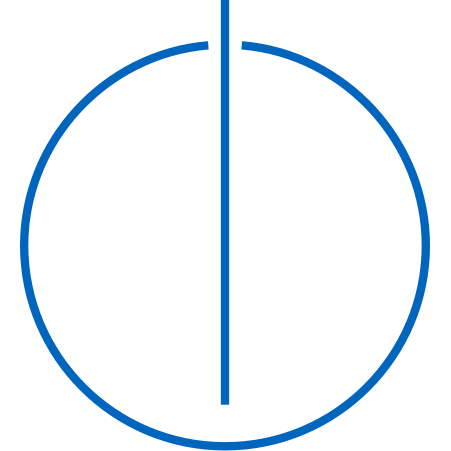
\includegraphics[height=20mm]{logos/faculty.png}
  }{}
\end{titlepage}


\frontmatter{}

\begin{titlepage}
  \centering

  \IfFileExists{logos/tum.pdf}{%
    
\includegraphics[height=20mm]{logos/tum.pdf}
  }{%
    \vspace*{20mm}
  }

  \vspace{5mm}
  {\huge\MakeUppercase{\getFaculty{}}}\\

  \vspace{5mm}
  {\large\MakeUppercase{\getUniversity{}}}\\

  \vspace{20mm}
  {\Large \getDoctype{}}

  \makeatletter
  \vspace{15mm}
  \ifthenelse{\pdf@strcmp{\languagename}{english}=0}
  {
  {\huge\bfseries \getTitle{}}

  \vspace{10mm}
  {\huge\bfseries \foreignlanguage{ngerman}{\getTitleGer{}}}
  }
  {
  {\huge\bfseries \getTitleGer{}}

  \vspace{10mm}
  {\huge\bfseries \foreignlanguage{english}{\getTitle{}}}
  }
  \makeatother

  \vspace{15mm}
  \begin{tabular}{l l}
    Author:          & \getAuthor{} \\
    Supervisor:      & \getSupervisor{} \\
    Advisor:         & \getAdvisor{} \\
    Submission Date: & \getSubmissionDate{} \\
  \end{tabular}

  \IfFileExists{logos/faculty.png}{%
    \vfill{}
    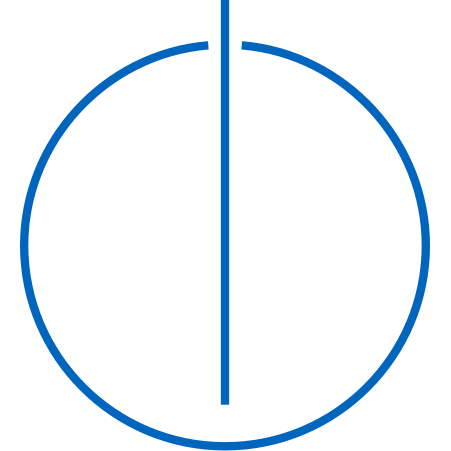
\includegraphics[height=20mm]{logos/faculty.png}
  }{}
\end{titlepage}

\cleardoublepage{}

\thispagestyle{empty}
\vspace*{0.8\textheight}
\noindent
\makeatletter
\ifthenelse{\pdf@strcmp{\languagename}{english}=0}
{I confirm that this \MakeLowercase{\getDoctype{}} is my own work and I have documented all sources and material used.}
{Ich versichere, dass ich diese \getDoctype{} selbstständig verfasst und nur die angegebenen Quellen und Hilfsmittel verwendet habe.}
\makeatother

\vspace{15mm}
\noindent
\getSubmissionLocation{}, \getSubmissionDate{} \hspace{50mm} \getAuthor{}

\cleardoublepage{}

\makeatletter
\ifthenelse{\pdf@strcmp{\languagename}{english}=0}
{\addcontentsline{toc}{chapter}{Acknowledgments}}
{\addcontentsline{toc}{chapter}{Danksagungen}}
\makeatother
\thispagestyle{empty}

\vspace*{20mm}

\begin{center}
\makeatletter
\ifthenelse{\pdf@strcmp{\languagename}{english}=0}
{\usekomafont{section} Acknowledgments}
{\usekomafont{section} Danksagungen}
\makeatother
\end{center}

\vspace{10mm}

Without doubt the very first name here is my father Musa Kazım Uzdoğan, who lost his fight to COVID-19 at the very beginning of this thesis. He with my mother Ayşegül Uzdoğan have been my biggest supporters throughout my life and put everything they had for me to become successful. Definitely, I am standing on the shoulders of giants. I know you would be extremely proud to see me achieve this. We will be loving and remembering you forever. I am also thankful for having a larger family who always showed their love and support through the difficult times.

Secondly, big thanks to my advisor Benjamin Sturm for his guidance and great communication throughout this work. I really enjoyed our discussions and appreciate your extensive feedback each time we met, although always virtually. I would also like to thank Prof. Ali Sunyaev and Prof. Jens Großklags for providing me the opportunity to work on this topic, and Tibor Posa for his reviews. Another mention goes to my colleagues at Max Planck Digital Library where I was working on the project bloxberg. Particularly to James Lawton, who introduced me to this problem and whom I enjoyed closely working with a lot. Also, I want to thank all interviewees for taking their time and providing valuable insights: João Pedro Oliveira, Tiago Paixão, Kevin Wittek, and two pseudonymous interviewees.

Finally, even though we never met, I want to commemorate Jon Tennant here, a great communicator and a tireless proponent of open science whose loss shocked many. I benefited and influenced by his works to a great extent, and the legacy he left helped me shape this work a lot. 

\cleardoublepage{}
 % TODO: if you don't have anyone to thank for or don't wish to publish it, comment this line out.
\chapter{\abstractname}

%TODO: Abstract


Hello World


\makeatletter
\ifthenelse{\pdf@strcmp{\languagename}{english}=0}
{\renewcommand{\abstractname}{Kurzfassung}}
{\renewcommand{\abstractname}{Abstract}}
\makeatother

\chapter{\abstractname}

%TODO: Abstract in other language
\begin{otherlanguage}{ngerman} % TODO: select other language, either ngerman or english !

\end{otherlanguage}


% Undo the name switch
\makeatletter
\ifthenelse{\pdf@strcmp{\languagename}{english}=0}
{\renewcommand{\abstractname}{Abstract}}
{\renewcommand{\abstractname}{Kurzfassung}}
\makeatother
\microtypesetup{protrusion=false}
\tableofcontents{}
\microtypesetup{protrusion=true}

\mainmatter{}

% !TeX root = ../main.tex
% Add the above to each chapter to make compiling the PDF easier in some editors.

\chapter{Introduction}\label{chapter:introduction}
Peer review is the formal process of the evaluation of scholarly works by people specialized in the subject of the work \parencite[p.~864]{Moxham.2018}. Common applications of peer review in scientific research are the selection of grant and fellowship applications, and the selection of manuscripts for scientific journals. In academic publishing when a researcher submits an academic paper for publication, journal editors ask “peers”, who are experts in the field to scrutinize the paper. Based on these reports the editor either rejects the paper, sends the paper back to the author for revision, or accepts it for publication. By determining what gets published or who gets funding, reviewers act as gatekeepers of science and the process ensures the quality and soundness of the scientific work \parencite{Bornmann.2011}.

\begin{figure}[htpb]
  \centering
  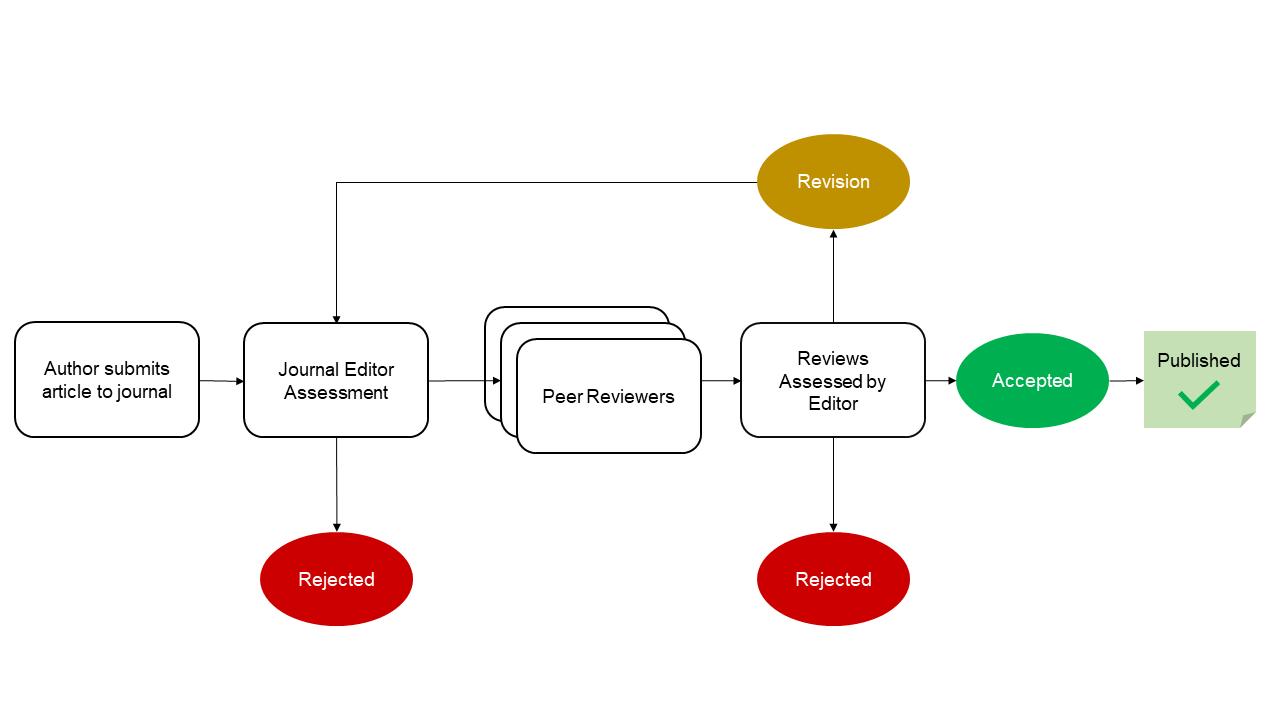
\includegraphics[width=0.8\textwidth]{figures/publishing-process.png}
  \caption{The publishing process} \label{fig:publishing-process}
\end{figure}

Peer reviews can be classified by how identities of parties are managed. In a double-blind review, only the editor knows the identities of the author and the reviewer. In a single-blind review, the name of the reviewer is hidden from the author to let the reviewer criticize without worrying about personal relationships or conflict of interests. The third and emergent form of the peer review is open peer review where the identities of both author and the reviewer are known to each other. In some forms of the open peer review, the identities and the review reports are also publicly available \parencite[4]{HorbachS.P.J.M..2017}, and therefore reviewers can gain credit for their work. Although, the term "open peer review" not only encompasses the openness of identities and the content, but also used for the open participation and transparency of the whole process \parencite{RossHellauer.2017}.

Peer review takes place in many different forms and employs different processes and it’s difficult to acknowledge it as a single system \parencite[2]{HorbachS.P.J.M..2017}. But its essence and rationale are shared among all different applications. Emerged among earlier scientific societies as an internal scrutinization for the scientific quality of manuscripts, it held its importance throughout the proliferation of the printing press, globalization of science after World War II \parencite{Fyfe.2017}, and the adoption of information technologies. It is still perceived by some as the gold standard in scientific publishing \parencite{Mayden.2012} and provides legitimacy for the generated knowledge \parencite{Tennant.2020c}.

\section{Problem Statement} \label{sec:problem-statement}

It is widely accepted that peer review plays an important role in research \parencite{Publons.2018, Taylor&Francis.2015, Ware.2008, Zuckerman.1971}. Despite its importance, peer review is shown to be far from being perfect, by being prone to biases \parencite{Lee.2013, Mahoney.1977}, inconsistencies \parencite{Peters.1982, Rothwell.2000}, and being ineffective in detecting errors \parencite{Schroter.2004}. It usually takes 3 to 5 hours (\cite[146]{Mulligan.2013}; \cite[42]{Ware.2008}) to complete a review and it usually takes more than 3 months for a paper to be accepted \parencite[51]{Ware.2008}. The process is often slow for authors and time consuming for reviewers. Reviewers who are academics themselves with various duties are often not compensated for their review work and they don’t receive credit for their work. Given that number of publications is growing each year \parencite{Bornmann.2015} and each manuscript typically requires 2 to 3 reviewers the peer review system is being put under growing pressure. This situation is said to cause “reviewer fatigue” \parencite{Breuning.2015}. At the same time, editors are reporting that it is getting more difficult to find suitable reviewers, indicated by the increasing decline rates to review invitations \parencite{Baveye.2011, Fox.2017}. 

Despite the numerous deficiencies of the process, it is argued that there is no consensus on an alternative \parencite{Smith.2006, Young.2003} and it is currently the best method ensuring the soundness of scientific publishing (\cite[5201]{Grainger.2007}; \cite[2]{HorbachS.P.J.M..2017}). A range of innovations aimed to tackle the stated problems failed to provide a cure and the peer review remains mostly unchanged \parencite{Tennant.2017}. 


\subsubsection{Peer Review Lacks Incentives}

Some of the problems of peer review are believed to be results of the lack of incentives to review \parencite{Derraik.2015, Willis.2016}, and there’s an ongoing discussion on how to increase researchers’ engagement in reviews in the light of these problems \parencite{Derraik.2015, Gasparyan.2015, Hauser.2007, Squazzoni.2013}. The lack of incentives has its roots within that today the measures and indicators of academic performance are the number of papers published, number of citations, or other citation based scientometrics. These measures play an important role in deciding who climbs up the ranks, who gets hired, or who receives the funding. Despite its importance, peer reviews usually are not recognized as a research output as the manuscripts and do not contribute to researchers’ perceived academic performance \parencite{Tennant.2017}. Therefore, researchers are disincentivized to do reviews and incentivized to publish more manuscripts.

The reliance on publishing-related metrics has also other consequences on peer reviewing. The state of affairs creates the mindset of “publish or perish”: the constant pressure to publish more and get cited more \parencite{Rawat.2014}. Yet, the way to publish more and get cited more is not only doing more research. One can publish the results of their work in smaller and less coherent slices \parencite[4]{Ferreira.2016} in an act called “salami publication” \parencite{SupakSmolcic.2013}. The act is considered unethical \parencite[238]{SupakSmolcic.2013} and with each paper reviewed by multiple reviewers, it puts more pressure on the peer review system \parencite[4]{Ferreira.2016}. This effect is amplified when a paper gets redundantly reviewed in different journals i.e. when authors go “journal shopping”. In this case, following a rejection by a journal with a higher impact, authors continue submitting their papers to gradually lower impact journals until their papers get published while the new editors and reviewers of the submitted paper are not aware of the previous reviews done \parencite[10]{Kovanis.2016}. 

If everyone publishes more and reviews less, then who is doing all the reviews? A strong imbalance in the peer review system was observed where a larger percentage of the peer reviews are done by a minority of researchers and thanks to them there is a sufficient supply of reviewers (\cite{Kovanis.2016}; \cite{Petchey.2014}; \cite[37]{Ware.2008}). Those “peer-review heroes” bear the burden by reviewing much more than they publish \parencite[9]{Kovanis.2016}. The situation raises the concerns that the system may be in a “tragedy of the reviewer commons” \parencite{Hochberg.2009} where participants of the system are encouraged to exploit the system by submitting more papers and less incentivized to do peer reviews. 

There’s a consensus among researchers that an improvement in peer review incentives would enable better reviews \parencite{Publons.2018}. Attracting more reviewers to the reviewer pool would also help balance the heavy burden placed on the reviewing system potentially letting editors find reviewers easier and shorten the time taken from submission until the publication of a manuscript. 

\subsubsection{Closedness of Reviews Prevents Their Acknowledgment}

The practice of blinded reviewing is a feature of the process that hinders public review acknowledgement. Today most of the peer reviews are done as single or double-blind \parencite{Wolfram.2020}. Even though open peer review seems to be gaining popularity \parencite{Wolfram.2020}, scientists are more likely to accept review requests when their identities are hidden \parencite{vanRooyen.1999} and majority of the researchers still prefer blinded reviews over open peer reviews (\cite[149]{Mulligan.2013}; \cite{Taylor&Francis.2015}; \cite[1038-1039]{Wolfram.2020}). It is likely the majority of peer reviews will remain blinded as the anonymity is considered necessary for strong and unbiased scrutiny \parencite[21-23]{RossHellauer.2017}.

However, a problem the closedness of reviews introduces is the difficulty to verify reviews. Since the whole review process takes place internally in journal management systems it is not possible to find out externally if a researcher has really done a peer review for a specific manuscript or a journal, without explicitly contacting the journal. In most of the cases, the transaction costs of contacting a journal is too large for a review, as virtually none of the journals has such a verification system. For reviewers to gain recognition for their work, it is essential that they can easily prove the authenticity of their reviews. The researchers may then showcase their review works done for specific journals and articles publicly or present them when needed as a demonstration of expertise in a field e.g. in job and grant applications. It may also highlight the reviewing workloads of researchers to their employers \parencite[2]{Raoult.2020}. 

Employers are increasingly resorting more to citation-based metrics for assessing their researchers \parencite{Bianchi.2019, Cantor.2015, Kachewar.2013, Verissimo.2013}. These metrics may be taken into account when assessing academic performance \parencite[11]{Ferreira.2016}. Availability of peer review contributions or related metrics may also bring incentives to do more reviews and reduce the imbalance in the review workloads \parencite[4]{Petchey.2014}. 

\subsubsection{Existing Peer Review Showcase Platforms Are Becoming the Sole Owners of Peer Review Data}

There are already running projects that aim to incentivize peer reviews by letting reviewers showcase their work. Since the review data is not publicly available, these "showcase platforms" can track the review contributions of a researcher for them, and verify the reviews they add to their profiles. By providing this verifications service, they act as a trusted third party between the reviewers and  and the bodies potentially interested in this information such as editors, funders, universities or agencies.

Reviewer Credits \footnote{https://www.reviewercredits.com}  is a project to let reviewers certify peer review activity, display their review records, and earn rewards such as books, and discounts to paid publishing services. Reviewers can claim their activity either through automated data transfer between the platform and journal or by Reviewer Credits manually contacting the publisher. \acrshort{ORCID}\footnote{https://orcid.org} also lets users add reviews to their profiles from open review journals or if the journal is an \acrshort{ORCID} member and provides review data to the platform though its \acrshort{API} \footnote{https://info.orcid.org/whats-new-with-peer-review-on-orcid/}. The more popular platform providing a similar service is Publons. Founded by Andrew Preston and Daniel Johnston in New Zealand in 2012 it quickly gained popularity and was welcomed by many academics \parencite[266]{Smith.2015} and was eventually acquired by Clarivate Analytics in 2017. As of November 2020, Publons claims to have over 2 million members\footnote{http://web.archive.org/web/20201109015743/https://publons.com/about/home}. On Publons, researchers can create a profile and add the reviews they have done. To add a peer review, they can either follow a link provided by the journal with a Publons integration after submitting their review or they can manually forward their review acceptance emails to Publons, who then manually verifies the review. By gathering publications and reviews, researchers can showcase their scholarly efforts and earn badges and awards such as “Top Reviewer” or “Highly Cited”. 

These platforms help researchers gain credit for their review contributions, but the proprietary status and of the review showcasing platforms and its potential implications may not be well aligned with the open science goals. Open science is a broad term used for different aspects of science and how science is conducted and there are different definitions of the term. \cite{VicenteSaez.2018} define it as knowledge generation with the four characteristics: transparent, accessible, shared, and collaborative by analyzing the use of term throughout the literature. \cite{Pontika.2015} created a taxonomy by braking down the the broader term "open science" into hierarchical components to provide a consistent terminology and to map the concepts around open science. \cite{Fecher.2013} identify five  schools of thought under the open science discourse, each aims for "opening" different aspects of the knowledge creation process. 

\begin{itemize}
    \item \textbf{Public School:} Open participation of the knowledge creation process, making science comprehensible for common citizens.
    \item \textbf{Democratic School:} Accessibility and transparency for the created knowledge: Open Access, Open Data
    \item \textbf{Pragmatic School:} Improving collaboration, stimulating knowledge dissemination.
    \item \textbf{Infrastructure School:} Providing researchers open tools for dissemination and collaboration 
    \item \textbf{Measurement School:} Finding new ways to measure researchers' impact, recognizing formerly invisible scientific contributions
\end{itemize}

Overall, open science aims to increase the rigour, accountability, and reproducibility in research and "to make research more open to participation, review/refutation, improvement and (re)use for the world to benefit" \parencite{Bezjak.2018}.

\begin{figure}[htpb]
  \centering
  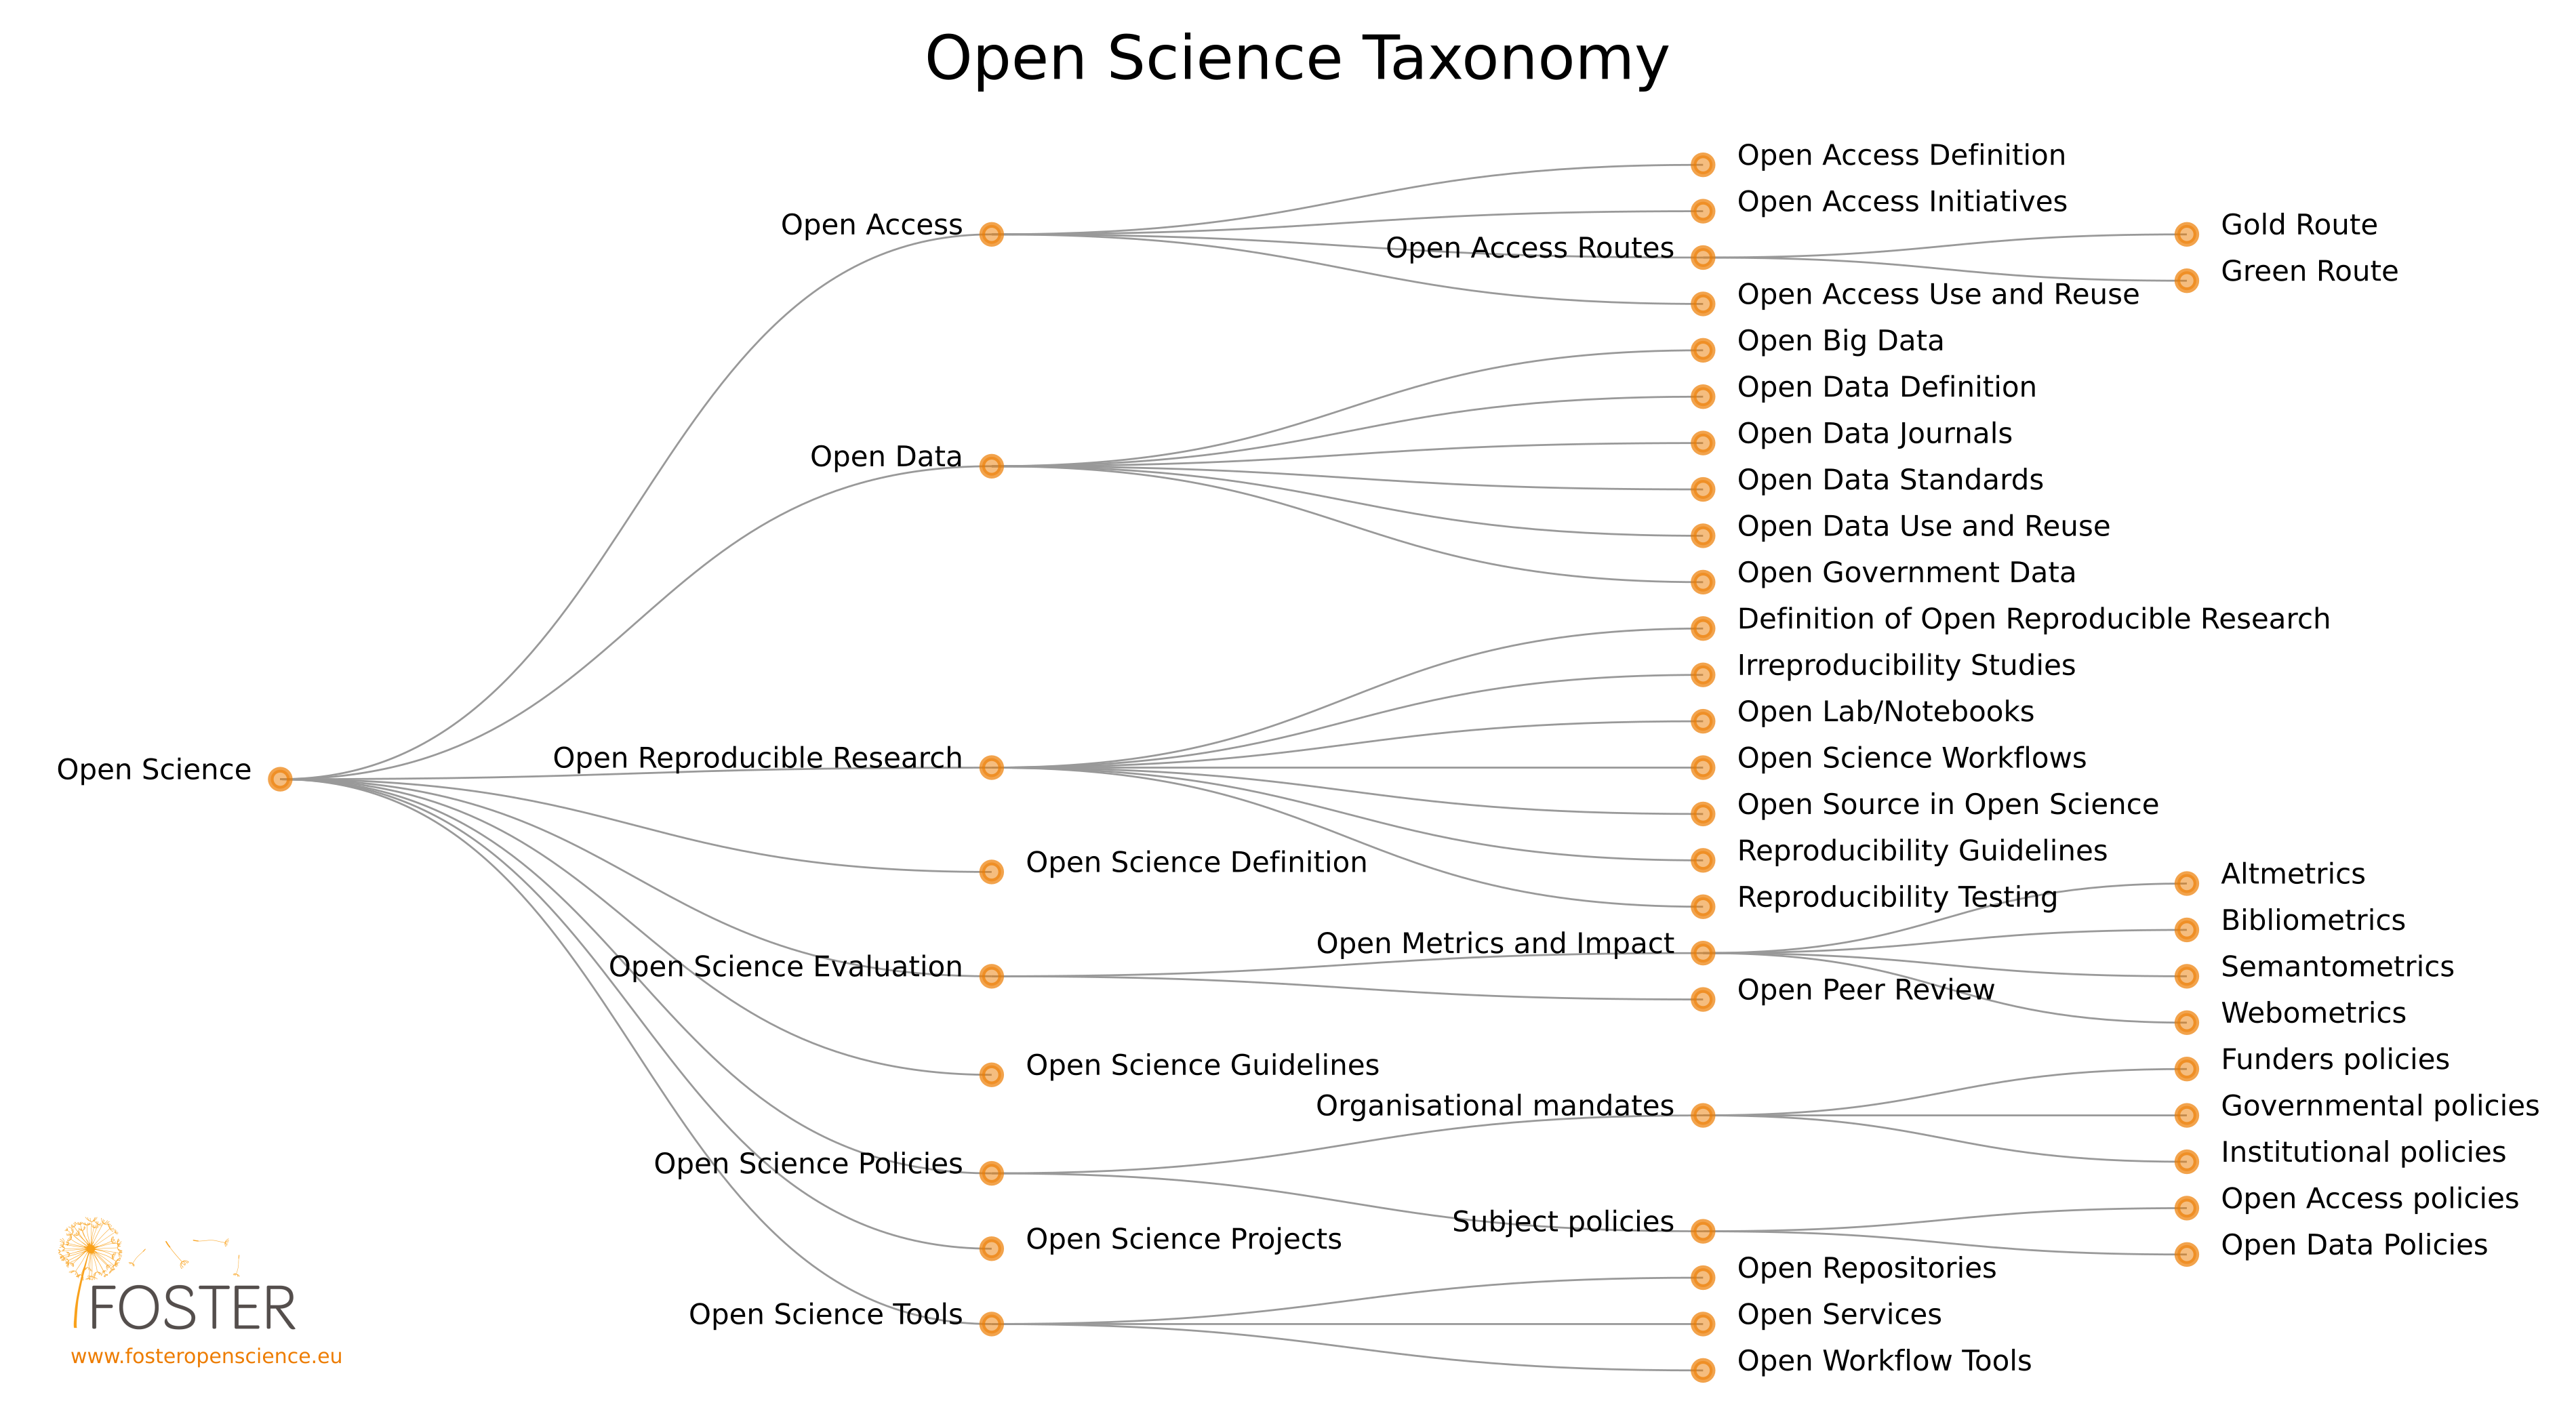
\includegraphics[width=0.8\textwidth]{figures/FOSTER.png}
  \caption{\parencite{Pontika.2015}} \label{fig:foster}
\end{figure}

Despite Publons being accepted by many scientists, it’s pointed out that its metrics may be biased \parencite{Ortega.2019}, and it may be failing to distinguish authentic reviews \parencite{TeixeiradaSilva.2020}. Current verification process by Publons, in particular the verification through review receipt emails, is not transparent. Publons lets users add reviews to their profiles by forwarding the "Thank you for your review" responses of journals. An email response is an easily forgable and unverifiable message. There are no studies on the peer review data if this problem is practically relevant, but there exist fake reviews \footnote{https://retractionwatch.com/2015/08/17/64-more-papers-retracted-for-fake-reviews-this-time-from-springer-journals/} \parencite{Qi.2017, TeixeiradaSilva.2017} and predatory journals wanting to exploit scientific metrics \parencite{xia2015publishes, demir2018predatory}, and credential fraud in science is well known \parencite{Wilson.2020}. Besides, on Publons it is not possible to see how the verification is done and there is no distinction on the platform between an email verification and a verification through a journal integration. Effectively, Publons has to be trusted for the data they provide.

Besides, the fact that the data on the platform is owned by Publons, and effectively Clarivate Analytics, brings the accessibility of the data into question. The platform’s provided API does not provide much data and existing studies making use of the Publons data extract it using web crawlers \parencite[952]{Ortega.2017} which is not allowed without Publons’ written consent according to the platform’s terms\footnote{https://web.archive.org/web/20210414004129/https://publons.com/about/terms/}. The platform appears to have provided data to researchers when requested \parencite[12]{Kovanis.2016}, however there are no guarantees that the data will remain freely accessible as long as it is owned by a proprietary company. Concerns have also been expressed for the transparency of the data previously provided by Clarivate Analytics (\cite{Rossner.2007}; \cite[3]{TeixeiradaSilva.2019}), as the provider of the Journal Impact Factor, and for the fairness of its practices \parencite{TeixeiradaSilva.2013}. A non-profit may be better suited for keeping this data open and accessible. But, currently in the case of \acrshort{ORCID}, which is a non-profit, the journals need to become paid \acrshort{ORCID} members and integrate their \acrshort{API} to be able write the review contributions of the researchers.

The aggregation of peer review data by proprietary parties might also be inappropriate for publishers and journals. The journals are effectively giving away their valuable review data to Publons for free. In turn, Clarivate Analytics processes this data and makes use of it for their profit. An example is the editor matching tool Publons has that lets editors find suitable matches for peer reviews of a manuscript\footnote{https://publons.com/benefits/reviewer-connect}. This itself may not be undesirable, as the fees may be justified by the value it provides for its users. But a single party aggregating the data has a higher risk of causing disagreements with publishers. If a publisher is unwilling to provide review data to a potential competitor, this may hinder the review coverage of the platform. Ideally, a platform should remain an open non-profit, or a joint organization governed by different stakeholders of the whole peer review ecosystem.

The problems of centralization in publishing is apparent \parencite{Lariviere.2015} and there is ever more demand for open science \parencite[1-3]{Piwowar.2018}. As long as the world’s peer review data is under the control of a single party, there exists the possibility for the sole owner of the data to restrict access to it, or start charging fees. This privileged position of the showcasing platforms are due to the role they play as trusted third parties in review verification. If these third parties can be disintermediated, and direct trust can be established between reviewers and consumers of the review data, a review showcasing system with more transparency, open standards, and open data may be possible.

\section{Research Question}

Peer review is a broad and controversial topic with many conflicting perspectives. The process also has many problems outlined that is interconnected with the other aspects of scientific epistemology and the current scientific publishing specifically. It is important to have a narrow focus to be able to analyze the specific problems and to bring impactful solutions. With the problems in peer review identified we focus on the implications of trusted third-parties in peer review verification and recognition and define the following as our research question: \\ 

\begin{center}
    \textit{How can closed peer reviews be verified without trusted third-parties?}
\end{center}

\section{Methodology}

As the work is exploratory and it is goal is to create an improved artifact that will enable the verification of closed peer reviews without a trusted third-party, it is suitable to structure the research process according to a design science framework. For this work the \acrfull{DSRM} proposed by \cite{Peffers.2007} is taken as a guideline for conducting research. The proposed framework presents a nominal process model that can be followed when conducting design science research in information systems. The authors suggest dividing the research process into 6 steps as shown in Figure \ref{fig:dsrm}. The process is not necessarily linear. During the research, the knowledge generated when creating the artifact can be used to refine and improve the artifact, and the improvement of the artifact yields more applicable knowledge. This cycle may be repeated multiple times until the artifact reaches the desired state. Additionally, it is possible to start the research process from the four entry points:

\begin{itemize}
    \item \textbf{Identify Problem \& Motivate:} Problem-Centered Initiation
    \item \textbf{Define Objectives of a Solution:} Objective-Centered Solution
    \item \textbf{Design \& Development:} Design \& Development Centered Initiation
    \item \textbf{Demonstration:} Client/Context Initiated
\end{itemize}

A problem-centered initiation is adopted for our research process. 

\begin{figure}[htpb]
  \centering
  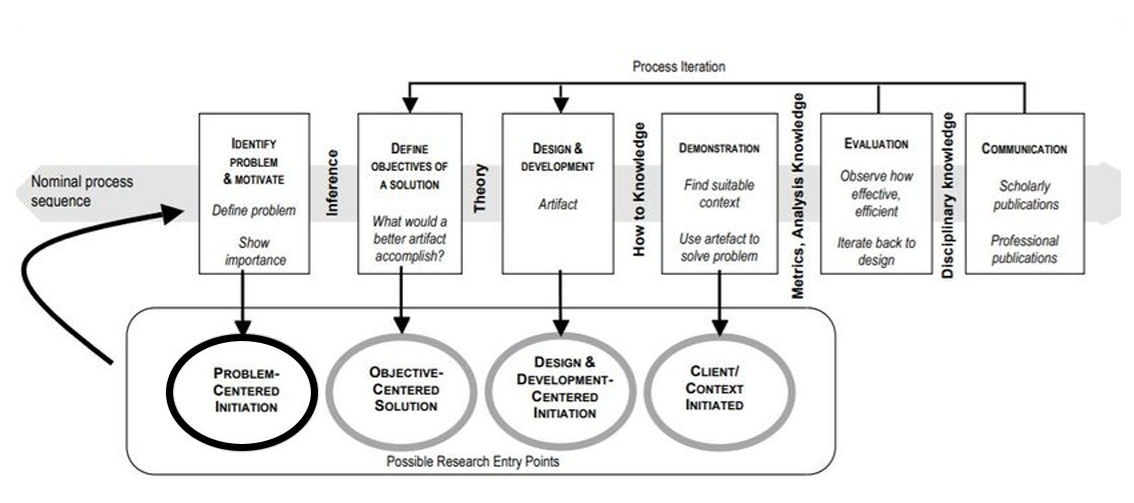
\includegraphics[width=\textwidth]{figures/dsrm.png}
  \caption{Design Science Research Methodology framework proposed by \cite{Peffers.2007}} \label{fig:dsrm}
\end{figure}

\subsubsection{Problem Identification}

We start with the problem identification where we take the \textit{peer review incentive problem}. The problem statement is given in detail in Section \ref{sec:problem-statement} but here we provide how our research brought us to the problems stated. The incentive problem encompasses that researchers are often busy with publication related work and, they are not incentivized to do voluntary peer reviews but instead are incentivized to publish more. This puts a burden on the reviewer resources available and this creates a typical tragedy of commons situation \parencite{hardin2009tragedy, Hochberg.2009} for the reviewer resources available. Further research in the literature uncovers the other problems in peer reviewing such as its quality, the long duration of the review process, and the increasing rejection rates, and that these problems can be traced back to the lack of incentives to do peer reviews. Solution proposals in the literature can be categorized in two groups: the ones that propose monetary incentives for doing peer reviews, and the proposals that focus on bringing recognition to the review contributions of researchers. The latter is also a benefit of open peer review that its proponents often state. This also shows the inherent dilemma of the peer review between keeping the reviews objective and unbiased, and making the process transparent and accountable, which stems from the practice of blinded reviews. Further, it reveals that the lack of recognition to peer reviews is due to the nature of the process, that the identities and contents of peer reviews are hidden and not shared publicly. Our research brings us to the platforms that aim to bring recognition to both open and closed reviews, namely the \textit{peer review showcasing platforms} e.g. Publons. 

Even though these platforms provide value to its users we identify some concerns about Publons. Also from an open science perspective and considering the practices of the centralized large publishers \parencite{Lariviere.2015} we identify problems related to transparency and centralization, and potential practices by the platform undesirable in terms of open data and open access. We pinpoint that these originate from the role these platforms take as \textit{trusted-third party} verifiers, and derive our main goal specifically from this. 

\subsubsection{Defining Objectives}

Considering the outlined problems, we define the main goal of the work as "How can closed peer reviews be verified without a trusted third-party?". Additionally, to design an artifact that achieves the main goal of the work, and to solve other specified problems we define a set of requirements (Section \ref{sec:requirements}) the designed artifact should satisfy. 

\subsubsection{Design and Development}

Based on the requirements we design the artifact using the \acrlong{VC} and \acrlong{zk-proofs} that allows the verification of closed reviews without a trusted third-party. We also describe a showcasing platform that allows the aggregation of reviews and lets researchers build a "peer review resume". We present the technical details of the designed artifact such as the defined peer review vocabulary and the conceived peer review credential. Additionally, we discuss the design decisions, and describe the main user flow in the system. 

\subsubsection{Demonstration}

We develop and deploy a working prototype as a proof-of-concept, and to demonstrate the technical feasibility of the artifact. We give an overview of the architecture of the prototype and demonstrate how users can interact with it. 

\subsubsection{Evaluation}

We evaluate the work qualitatively through interviews with academics that are familiar with the peer review process and the peer review showcasing platforms.

%% TODO: TAM framework

\subsubsection{Communication}

Finally, the work is communicated in the form of a thesis document, and the open source code is shared on \href{https://github.com/kuzdogan/peer-review-verifiable-credentials-thesis}{GitHub} with instructions how to use the deployed prototype. 


\section{Related Work}

The problems in peer review caught the attention of scientists. Besides the descriptive literature on peer review’s shortcomings, a variety of works discussed and prescribed solutions to the incentive problem. An often encountered suggestion is to ask researchers to do sufficient reviews to balance the system, usually 3 reviews per paper, a “quid pro quo” (\cite{Derraik.2015}, \cite[5201]{Grainger.2007}). To maintain the timeliness of the process \cite{Hauser.2007} suggest a punishment for reviewers who return their reviews late and a reward for the ones returning on time. \cite{Ferreira.2016} suggest making peer review mandatory and paying the reviewers and calls for a decoupling of the peer review system from the scientific publishing by founding a Global Peer Review Platform. Direct monetary compensation of reviewers was also suggested many times \parencite{Prufer.2010}. \cite{Fox.2010} suggest a credit system where authors have to pay for their submissions and earn by conducting reviews, effectively “privatizing the reviewer commons”. Others proposed crypto-economic models through peer review tokens on a blockchain that will work as credits for peer reviews or as reputation indicators \parencite{Avital.2018, Jan.2018c, Spearpoint.2017, Tarkhanov.2020}. Also using a blockchain-based token and lotteries \cite{Janowicz.2018} provide a model for how integrating distributed ledger technologies could benefit the Semantic Web journal’s processes. \cite{TenorioFornes.2019} suggest a whole publishing system that is decentralized using Ethereum and IPFS. Ants-Review suggests an Ethereum based incentive system with its native token ANTS that allows bounties for open anonymous peer reviews \parencite{TrovoMassari}.

\section{Structure}

The rest of this work is structured as follows: \hyperref[chapter:background]{Chapter 2 (Background)} introduces the technical foundations in this work that are required for the creation of and to understand the proposed solution. \hyperref[chapter:design]{Chapter 3 (Design \& Implementation)} outlines the requirements defined for the designed artefact and describes the design of the proposed system. Here the details of the artefact are laid out and the design decisions are communicated. Next in this chapter, the implemented prototype is described, which demonstrates the technical feasibility of the conceived design. A comparison between the conceptual design and the implemented prototype is also provided. \hyperref[chapter:evaluation]{Chapter 4 (Evaluation)} involves the evaluation of the designed artefact based on the interviews with researchers. \hyperref[chapter:discussion]{Chapter 5 (Discussion)} shares the learnings gained in the process, and discusses potential future work and considerations. Finally, \hyperref[chapter:conclusion]{Chapter 6 (Conclusion)} presents the conclusions.
% !TeX root = ../main.tex
% Add the above to each chapter to make compiling the PDF easier in some editors.

\chapter{Background}\label{chapter:background}

\section{Verifiable Credentials}

\acrfull{VC} is a recent \acrshort{W3C} standard "to express credentials on the Web in a way that is cryptographically secure, privacy respecting, and machine-verifiable" \parencite{Sporny.18Kas2019}. These credentials include but are not limited to passports, ID cards, university degrees, tickets etc. Any set of claims about a subject can be a credential. In the \acrshort{VC} setting these claims create \textit{subject-property-value} relationships that can be expressed in graphs. For instance being graduated from a university can be represented as the graph in Figure \ref{fig:alumniOf}. 

Subjects of claims are not necessarily persons and can be anything. In a peer review context a claim could be \textit{Peer Review-author-John Doe} where the subject is the peer review. Alternatively same relationship can be represented as \textit{John Doe-reviewerOf-Peer Review} where the subject is the person.

\begin{figure}[htbp]
  \centering
  \includesvg[width=0.8\textwidth]{claim-example}
  \caption{Example Subject-Property-Value relationship of a graduation claim \parencite{Sporny.18Kas2019}} \label{fig:alumniOf}
\end{figure}

Although people usually associate credentials to be issued only by a respected authority such as a state, a university or a hospital, \acrlong{VC} allows anyone to issue claims. Yet, each credential is meaningful in a certain context and depending on the trust relationships between parties. An \textit{alumniOf} claim is only meaningful if issued by a university that is known to the employer in a job application or a \textit{goodHusband} claim only makes sense if issued by a spouse. Parties that receive a credential can choose to accept or reject a credential depending on the real world trust relationships.

A credential is a set of claims, i.e. a graph of information around a subject. Additional to the claims, the metadata and a digital proof form a verifiable credential. The proof is generally a digital signature of the claims and metadata, which makes the verifiable credential "verifiable".

\begin{figure}[htbp]
  \centering
  \includesvg[width=0.4\textwidth]{credential}
  \includesvg[width=0.8\textwidth]{credential-graph}
  \caption{Components of a verifiable credential and the graph of information of an example credential \parencite{Sporny.18Kas2019}} \label{fig:credentialGraph}
\end{figure}

The \acrshort{VC} specification models the stakeholders and interactions between them as in Figure \ref{fig:ecosystem}. \textit{Issuer}s assert claims and issue credentials about subjects, \textit{Verifier}s verify the credentials presented to them, and \textit{Holder}s aquire, store, and present credentials. Note that the subject of a credential can be different than its holder such as a pet being the subject and its owner being the holder, or a peer review as the subject and the reviewer as the holder. Finally, a \textit{Verifiable Data Registry} acts as the backend of these interactions by maintaining identifiers and schemas. This registry could be a distributed ledger or a central database depending on the implementation.

\begin{figure}[htbp]
  \centering
  \includesvg[width=0.8\textwidth]{ecosystem}
  \caption{Stakeholders of a \acrlong{VC} ecosystem and their roles \parencite{Sporny.18Kas2019}} \label{fig:ecosystem}
\end{figure}

\subsection{Verifiable Presentations}

The specification also describes an extension to the \acrshort{VC} data model that enables the packaging of multiple credentials and verification of the authorship of the data. A Verifiable Presentation consists of one or more verifiable credentials, presentation metadata, and a proof which is usually a digital signature of the first two. Credential holders can combine different credentials from different issuers for each use case, and the proof of the presentation provides the means to verify the authorship of data.

\subsection{Syntax}

The data model provided in the \acrshort{VC} specification is an abstract representation of the information around a credential. For the exchange of the information a machine readable data exchange format or syntax is required. Popular data exchange formats are XML \parencite{xmlRFC}, \acrshort{JSON} \parencite{jsonRFC}, and \acrshort{YAML} \parencite{yaml}. Although any syntax can be used, the specification describes \acrshort{JSON} and \acrshort{JSON-LD} \parencite{jsonld} serializations of the data model. 

The use of linked data through \acrshort{JSON-LD} accomplishes several things. First, it  brings linked data properties with minimal changes to \acrshort{JSON}, which is widely used in today's web. Second, it makes possible to model complex real world relationships with a graph model. Third, it enables "permissionless innovation" through extensibility. Anyone can extend the existing vocabularies and numerous cryptographic proof formats and signature suites can be used. This is in line with the "open world assumption" approach, that is anyone can assert claims about any subject. It is up to implementers and verifiers to decide based on the real world trust relationships which claims to accept and which entities to trust. Other benefits of \acrshort{JSON-LD} over diferrent formats in \acrlong{VC} is discussed in \cite{young_2021}. 

A minimal verifiable credential in \acrshort{JSON-LD} format is shown in Listing \ref{lst:exampleVC}.

\lstinputlisting[language=json, caption={Example verifiable credential \parencite{Sporny.18Kas2019}},label={lst:exampleVC}]{code/exampleVerifiableCredential.json}

Originally, keys in \acrshort{JSON-LD} documents are \acrfull{IRI}s \parencite{rfc3987}, which are similar to \acrfull{URI}s \parencite{rfc3986}. This lets machines to unambiguously refer things in the world. For instance the meaning of the property \lstinline{children} may be obvious for a human-reader depending on the context. If the reader sees the property under a person, they can infer it means a son or a daughter of that person. However, \lstinline{children} is also used to express hierarchical relationships between things. These semantics need to be stated explicitly for machines to be able to "understand" what these properties stand for and to avoid such ambiguities in machine communication. That's why instead the keys are \acrshort{URI}s. Also to avoid everyone defining their own \lstinline{child} semantics, vocabularies are defined. One popular vocabulary is \url{schema.org}. To express "a child of a person", the \acrshort{IRI} \url{https://schema.org/children} can be given. In that case a \acrshort{JSON-LD} document looks like in Listing \ref{lst:exampleJSONLD}

\begin{lstlisting}[language=json, label={lst:exampleJSONLD}, caption={A JSON-LD with full \acrshort{IRI}s}]
{
  "http://schema.org/givenName": "John",
  "http://schema.org/familyName": "Doe",
  "http://schema.org/children": {
    "@id": "http://doefamily.net/jane",
    "http://schema.org/givenName": "Jane",
    "http://schema.org/familyName": "Doe"
  }
}
\end{lstlisting}

Instead of having to write full \acrshort{IRI}s each time, a \lstinline{@context} can be included in the document that will map terms in the included document to \acrshort{IRI}s. Similar to a human communication, this sets the context of the information exchange, thus removing the ambiguity. A context document for the previous \acrshort{JSON-LD} file might be as follows

\begin{lstlisting}[language=json, label={lst:exampleJSONLD}, caption={A context file}]
{
  "@context": {
    "firstName": "http://schema.org/firstName",
    "lastName": "http://schema.org/lastName",
    "children": "http://schema.org/children"
}
\end{lstlisting}

Assuming the context is located at \lstinline{http://example.com/familyContext}, the previous document becomes more human-readable by embedding the context.

\begin{lstlisting}[language=json, label={lst:exampleJSONLD}, caption={A context added JSON-LD with shortened terms}]
{
    "@context": "http://example.com/familyContext",
    "givenName": "John",
    "familyName": "Doe",
    "children": {
        "@id": "http://doefamily.net/jane",
        "givenName": "Jane",
        "familyName": "Doe"
    }
}
\end{lstlisting}



\section{Zero-Knowledge Proofs}

Zero-knowledge proofs of knowledge are protocols in cryptography where a \textit{prover} can cryptographically prove to a \textit{verifier} the validity of statement without sharing any other information than the fact that the statement is true. The field recently received more attention with the implementation of the privacy-preserving digital currency Zcash \parencite{E.BenSasson.2016}. Even though commonly referred as zero-knowledge proofs, it is useful to distinguish between \textit{proofs} and \textit{proofs of knowledge}. A proof is sufficient evidence for the truth of a proposition such as a proof for the statement that there exists a three coloring for a specific graph. A proof of knowledge is a proof for the knowledge of a piece of information such as a proof to the statement that I know a three coloring for this specific graph \parencite{green_2017}. 

Properties of zero-knowledge proofs are as follows \parencite{Groth.2010}:
\begin{itemize}
  \item \textbf{Completeness:} If the statement is true, the verifier will be convinced by the proof the prover presents that the statement is true
  \item \textbf{Soundness:} If the statement is false, a malicious prover can't convince the verifier that it is true.
  \item \textbf{Zero-Knowledge:} If the statement is true, a malicious verifier does not learn anything else than the fact that the statement is true.
\end{itemize}

The first two properties are also requirements for interactive proofs. The work of \cite{Goldwasser.1985} has first introduced the third property of Zero-Knowledge. A proof in a zero-knowledge proof system is not deterministic but a probabilistic proof. Through many rounds it is possible to decrease the error to practically negligible values. \cite{Goldreich.1991} also show that with the assumption of an unbreakable encryption, it is possible to create a zero-knowledge proof for the graph coloring problem. This is significant since the graph coloring problem is NP-complete and every NP problem can be reduced to an NP-complete problem in polynomial time, meaning every problem in NP has a zero-knowledge proof. 

These initial zero-knowledge proofs are also interactive, that is the prover and the verifier need to exchange information on each round. Each time the a proofs needs to be made, the prover and the verifier need to be online and interact in multiple rounds, which makes the usability of the protocol difficult. Also, since the soundness of the proof relies on the randomness of the challenges of the verifier on each round, a third-party can not be convinced by such a proof. By looking at the protocol transcript and the proof, they can't be assured if this randomness holds. \cite{Blum.1988} have shown that with a common reference string shared by the prover and the verifier, it is possible to create non-interactive zero-knowledge proofs. The common reference string need not be private, which makes non-interactive zero-knowledge proofs more practical than interactive ones.

\section{Related Work}
% !TeX root = ../main.tex
% Add the above to each chapter to make compiling the PDF easier in some editors.

\chapter{Design and Implementation}\label{chapter:design}

The goal of this work is to design a system that will allow the verification of closed peer reviews without a trusted third party. The new artifact should improve upon the existing ones, which are the current peer review showcase platforms. Based on the problems identified, the requirements of such a system is defined in the following section. Taking these requirements and available technologies into account, a design of system will be communicated. Additionally, the implemented proof of concept prototype will be demonstrated.

\section{Requirements} \label{sec:requirements}

Following the open science principles, this information should be as transparent and accessible as possible. However, the anonymous nature of the review process does not allow this. 

As stated in the problem statement, current lack of recognition of peer reviews stems from the public unavailability of the closed peer reviews. Each individual party presented with the peer reviews of a researcher needs to explicitly contact each journal if they want to verify the peer reviews. This is clearly infeasible in a public setting: if a researcher has their peer reviews stated in a public profile, e.g. on their website, each party consuming this data has to contact the journals. This is not the case for other scholarly works such as manuscripts. Therefore, it should be easy to check if the peer review is authentic, that is, the peer reviews are \textbf{verifiable}.

Currently, there are platforms for aggregating and showcasing peer reviews. The process of adding peer reviews to these platforms include automatic methods such as integrations with journals. Users can also add reviews manually such as by sending the review receipt emails or by filling out the review information on the platform. These will get checked by the platform and then the peer review will be "verified". However, it is not possible to trace how the the review is verified and it is at the platforms discretion to decide what constitutes a verified review and what is not. There are researchers on these platforms that have over 1000 verified reviews per year on their profile. Questions about the validity of this data has been raised \parencite{TeixeiradaSilva.2020, TeixeiradaSilva.2017, TeixeiradaSilva.2019}. Following the open science principles it is important to provide provenance on data and \textbf{transparency} on how the verification is done.

It is outlined in previous sections, how the review showcasing platforms aggregate review data by acting as trusted third-parties. They become the sources of peer review contributions of a researcher and decide what is a "verified" review. The data stored by the platforms is different than what is available to public, which enables potentially putting the data behind a paywall or charging its users. Therefore, \textbf{open data} is another requirement of the system. In parallel, by having a system design based on \textbf{open standards}, vendor lock-in can be avoided. This lets anybody provide review showcasing services and users will have the freedom to choose which service they want to use. Also, the platforms' ability to hold onto the peer review data is provided by their position as the trusted third-parties.  Instead, it is desirable to create direct trust between the parties. The designed system should facilitate \textbf{direct trust} between the stakeholders. 

A peer review has various metadata associated. The necessary data to be presented may be different in each context. For a review author it is useful to be able present different data associated with the review without breaking the verifiabilty of the review. For instance, the contents and the date of a closed review may not be shared on a public profile, but a review author might want to share these in a more private setting such as in a job or grant application. In both cases, the reviewer should be able to \textbf{selectively disclose} which attributes they want to share.

Peer review practices vary a lot between fields, even from journal to journal within the same field. Hence, the required system should be \textbf{compatible} with the different practices and different data resulting from these processes. The system should enable the creation of different data schemas, but at the same time avoid ambiguity and let stakeholders communicate what this data means.

Here the requirements are listed together once again.
\begin{itemize}
  \item RQ1: Verifiability \label{rq:verifiable}
  \item RQ2: Transparency \label{rq:transparent}
  \item RQ3: Open Data \label{rq:open-data}
  \item RQ4: Open Standards \label{rq:open-standards}
  \item RQ5: Direct Trust \label{rq:direct-trust}
  \item RQ6: Selective Disclosure \label{rq:selective-disclosure}
  \item RQ7: Compatibility \label{rq:compatible}
\end{itemize}

\section{Design}

%% TODO: Why I choose JSON-LD over JWT see https://www.w3.org/TR/vc-imp-guide and Kaliya Young's doc
% "The relying party (verifier) is left guessing about the meaning, and if they don’t want to guess, they must find an out-of-band way to connect back to the issuer to figure out the meaning."

% Why is the review the subject
% Because it is "the" credential. We make a Peer Review Credential. A peer review authorship credential is trivial.

% We don't care how the credential is transferred. g DIDComm, pairwise connection using JWT, SIOP CHAPI etc.

\subsection{Overview}

We choose to base our design on W3C's Verifiable Credentials specification \parencite{Sporny.18Kas2019}. The specification inherently satisfies some of the requirements of our system. It is verifiable, based on open standards, and built with an open world assumption, that is, anyone can extend the existing vocabularies and can issue credentials. Also, there exist open source \acrshort{VC} libraries that can be used in the implementation.

The designed system has two main components:

\begin{enumerate}
    \item \textbf{Journal X:} A hypothetical journal that issues peer review credentials
    \item \textbf{Veriview:} A peer review showcase platform that supports VC
\end{enumerate}


In a typical peer review process, a researcher receives an invitation to do a peer review from the editor of the journal. Here, upon receiving an invitation from Journal X, the reviewer accepts it and submits the review of the manuscript to Journal X. Then she can request the proof of their work as a peer review verifiable credential. Journal X prepares the credential and issues it by signing the document. The review author can use this credential to prove their authorship. In our system we also conceive a peer review showcasing platform called Veriview, where review authors can build their "peer review resume". According to the privacy policy of the review, they can decide which information about the review to share publicly. For instance, a blinded review typically can't be shared with identifiable information such as the manuscript, the content, the title etc. The reviewer is able to choose which information to share on their public profile accordingly. An overview of the interactions of the typical use case on the system are depicted below in Figure \ref{fig:sequence1} 

\begin{figure}[htpb]
  \centering
  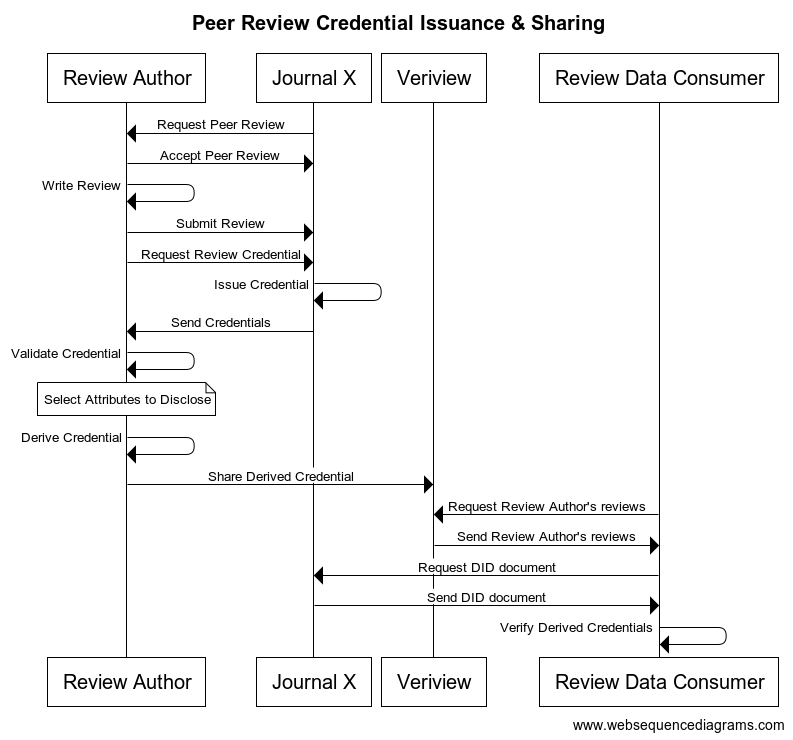
\includegraphics[width=0.8\textwidth]{figures/sequence.png}
  \caption{Overview of peer review credential issuance and sharing process} \label{fig:sequence1}
\end{figure}

In practice, there supposed to be many journals and Journal X is one example out of numerous journals. Also Veriview is not a single platform but there may be many showcasing platforms that researchers can choose to build their profiles at. Having a system based on open standards \hyperref[rq:open-standards]{(RQ4)} allows anyone to create a platform similar to Veriview and this would avoid vendor lock-in. 

Additionally we assume a "Review Data Consumer", a party which is interested in the peer review data of a reviewer. In real world these might be employers, universities, research institutions, or other researchers. Any party that is interested in the peer reviews of a researcher, and their authenticity, might be a consumer. 

The use case depicted in Figure \ref{fig:sequence1} assumes the reviews are shared publicly and are not open reviews. Since Veriview is a platform to share peer reviews publicly, the review author will choose which attributes they want to and are able to share, and derive a credential containing the selected attributes and a zero-knowledge proof which can be shared in Veriview. 

In a private setting or for an open review this additional derivation step is not required. For instance, if the researcher wants to include their review in a grant application, they might want to share the reviewed manuscript and the contents of the review. If the manuscript is in the scientific field the researcher wants to show competence in, being able to verifiably show that they were invited and done a review in this field  would demonstrate the researcher's competence. Also, other factors such as the journal's reputation provide additional information. In this case Veriview is not required and the interactions are as in Figure \ref{fig:sequencePrivate}.

\begin{figure}[htpb]
  \centering
  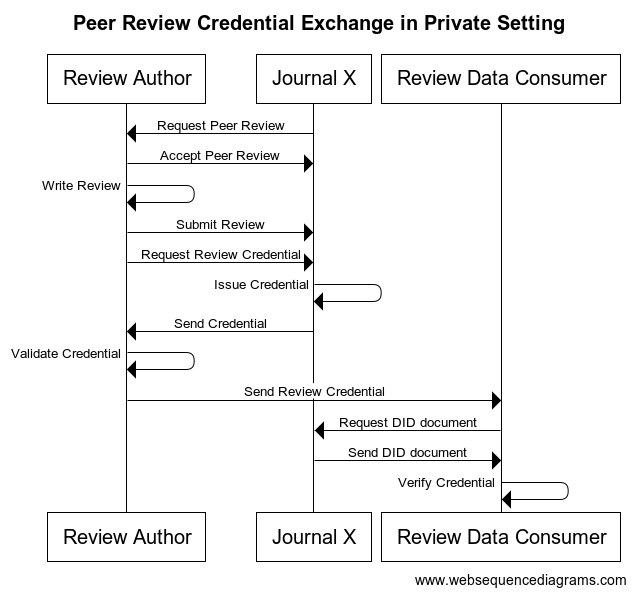
\includegraphics[width=0.8\textwidth]{figures/sequencePrivate.png}
  \caption{Peer Review Credential Exchange in a Private Setting} \label{fig:sequencePrivate}
\end{figure}

\subsection{Peer Review Credential}

The Peer Review Credential is a document issued by a journal that a peer review has been done for this journal. The document contains the review content and the metadata associated such as the date, title, author etc. An example credential is given below in Listing \ref{lst:exampleReview}

\lstinputlisting[language=json, caption={Example Peer Review Credential},label={lst:exampleReview}]{code/exampleReviewCredential.json}

The credential in this design follows the \acrshort{JSON-LD} syntax. \acrshort{JSON-LD} is the predominantly used format in the \acrshort{VC} specification. It is also an open standard under W3C \parencite{jsonld} \hyperref[rq:open-standards]{(RQ4)} and many of the \acrshort{VC} libraries available are \acrshort{JSON-LD} based.  \acrshort{JSON-LD}s with Linked Proofs supports Zero-Knowledge Proof formats and \acrshort{JSON-LD}s require canonicalization, which allows flexibility in the order of the attributes. This becomes useful for instance when transferring the credential from the journal to the author, the journal doesn't have to worry about the order of the attributes when they issue the credential. Also, being fully compatible with \acrshort{JSON}, the format easily integrates with existing web frameworks. 

The credential is designed to represent the review as the subject. Under the \lstinline{credentialSubject} the data related to review is contained, including the \lstinline{author} field which represents the author of the review. An alternative representation could be to issue a "review authorship" credential which would contain the author as the credential subject and an \lstinline{authoredReview} field containing the review data. Both are valid expressions of the same relationships, but here it is chosen to represent the review itself as the system is for "peer review credentials" and a peer review credential implies the review itself is the credential being issued. In the other case, it is needed to express the credential as a "peer review authorship credential" explicitly and this might create confusion.

\subsubsection{Context}

\lstinline{@context} defines the vocabularies used in the document. The first \acrshort{URL} refers to the \acrshort{VC} context and it is required to be included in all verifiable credentials according to the specification. The second context contains the vocabulary for peer reviews. Finally, \lstinline{https://w3id.org/security/bbs/v1} provides the vocabulary for the \lstinline{BbsBlsSignature} signature suite since it is not included in the default \lstinline{https://www.w3.org/2018/credentials/v1} context. We also provide a vocabulary for our system specific for the peer reviews. The context used in this document is given in Listing \ref{lst:peer-review-context}

\lstinputlisting[language=json, caption={Peer Review Vocabulary},label={lst:peer-review-context}]{code/peerReviewContext.json}

The vocabulary document itself is a context that defines three different contexts, namely \lstinline{PeerReviewCredential}, \lstinline{PeerReview}, and \lstinline{PeerReviewAuthor}. These contexts can be included in the corresponding objects in the credential by adding to the \lstinline{type} field in the \acrshort{JSON-LD} credential document. The \lstinline{@version} term defines the \acrshort{JSON-LD} version of the definition. This will explicitly tell the \acrshort{JSON-LD} processor to use the version 1.1 processing mode. It is not a requirement to set the version explicitly but this practice avoids potentially processing the document with the older \acrshort{JSON-LD} processors. 


In the vocabulary, terms from \url{schema.org} was used when there exist a clearly overlapping term in the schema.org ontology, such as the \acrshort{ISSN} field or the title field which corresponds to \url{schema.org/headline}. In other cases, self-referring definitions are made, which refer to themselves in the \lstinline{@id} field, as in the case with the \lstinline{author} or \lstinline{journal} fields. There exists a term for \lstinline{author} in schema.org but we prefer the schema to be explicit and to be included in credential document through adding the \lstinline{PeerReviewAuthor} in the \lstinline{type} field. Similarly, an explicit definition of \lstinline{journal} is preferred over the general \lstinline{schema.org/Periodical} term. Also, by defining the term \lstinline{"schema": "http://schema.org/"} it is made possible to map the \acrshort{URL} paths to the schema.org. As an example, this allows \lstinline{schema:name} to be expanded into \lstinline{http://schema.org/name} when processed. 

The previous version of the defined peer review vocabulary included \lstinline{@protected: true} attributes in \lstinline{@context}'s, which prevents overriding attributes by new definitions. Even though this adds extra protection to term definitions, it disallows the extension on the definitions. It is removed to enable extensibility. The peer review process varies a lot at each publisher or journal, and issuers can adopt the vocabularies according to their needs. The vocabulary assumes a basic credential model with few attributes associated with a peer review. Thanks to the extensibility of \acrshort{JSON-LD} vocabularies, it possible to extend the vocabulary itself, or include other vocabularies in the document. For instance, if the peer review process of a journal has a statistical soundness check, this can be represented as a \lstinline{statisticallySound} field defined in another vocabulary and included in the credential context. This enables the compatibility of the system \hyperref[rq:compatible]{(RQ7)} with different peer review processes.  Ideally, these vocabularies will be defined with different stakeholders of the peer review ecosystem coming together, that they will be widely accepted and used.


\subsubsection{Signatures}

We choose BBS+ signatures with a BLS12-381 curve as expressed by the \lstinline{BbsBlsSignatureProof2020} type in the \lstinline{proof} field. BBS+ signatures is the preferred signature scheme while BLS12-381 is the curve used for generating the keys. BBS+ signatures can be used with any pairing friendly curve \parencite{irtf-cfrg-pairing-friendly-curves-09}, but since the existing Linked Data Proof signature suite \parencite{looker_steele_2021} and the implementations\footnote{https://github.com/mattrglobal/bbs-signatures-spec} are based on BLS12-381 curves, we choose adopt the same curve. This signature suite allows zero-knowledge selective disclosure of attributes \hyperref[rq:selective-disclosure]{(RQ6)} with more efficient size and execution times\footnote{https://docs.google.com/presentation/d/1JRzlzS3Y3NTm_NPzxlnud7xIDmGL_9aHHX55MMwvtlU} compared to the existing ones such as \acrshort{CL} signatures. 

With BBS+ signatures it is possible to sign multiple messages. The signature scheme provides a $sign$ and a $verify$ verify function that are also found in other digital signature schemes. The signature is not over the whole message and the size of the signature is variable with the number of messages hidden. For an array of messages $m[0], m[1], ..., m[n]$, a public key $privk$, a private (secret) key $pubk$ the below functions are provided.

\[signature = sign((m[0], m[1], ..., m[n]), pubk, privk)\]

\[result = verify((m[0], m[1], ..., m[n]), signature, pubk)\]

Where result is a boolean value representing the validity of the signature. Additionally, the BBS+ signatures allows derivation of a \textit{proof} of knowledge of the original signature and the verification of the proof. A party who knows the messages, the public key, and the signature over all of the messages can take a subset of the messages and create a zero-knowledge proof as follows:

\[proof = derive( (m[3], m5],..., m[n-1]), signature, pubk)\]

Which can be verified with: 

\[result = verifyProof( (m[3], m[5],..., m[n-1]), proof, pubk) \]

With the BLS12-381 curve the element sizes are as follows\footnote{https://github.com/mattrglobal/bbs-signatures}:
\begin{center}
\begin{tabular}{ c c }
  Element & Size    \\
  \hline
  $privk$   &   32 bytes    \\
  $pubk$    &   96 bytes    \\
  $signature$ & 112 bytes   \\
  $proof$   &   368 + (hidden message count) x 32 bytes
\end{tabular}
\end{center}

\subsubsection{Decentralized Identifiers}

The \acrshort{VC} specification describes several attributes as identifiers (i.e. \acrshort{URI}s). Apart from uniquely identifying the described object, these fields may also be used for authentication. In the case of \lstinline{issuer}, the value of the attribute is recommended to resolve to a document that can be used to verify the credential. The document would contain the public key information of the signer key, and other meta-data related to the issuer. Similarly, a \acrshort{DID} in the \lstinline{author} field can be used for verification in a credential exchange. The holder of the credential (author) can wrap the credential or multiple credentials in a verifiable presentation to ensure it is being sent from the intended holder. 

In this system, the issuer field is a \acrshort{DID} of the journal. It is required for the verifiablity of the peer reviews to have this identifier field resolve to a document with a public key \hyperref[rq:verifiable]{(RQ1)}. Although it is possible to use an \acrshort{HTTP} \acrshort{URL} that resolve to a document containing public keys, we use \acrshort{DID}s since it provides a standard document format that can be used for verification, and for their close relationship with \acrshort{VC}s in the \acrshort{SSI} ecosystem. 

Using a \acrshort{DLT} based \acrshort{DID} method would provide the document a high availability, tamper-proofness, and won't require to contact the issuer at each verification. An example would be \lstinline{did:sov:mnjkl98uipsndg2hdjdjuf7} which represents a DID that can be resolved with the Sovrin blockchain method. However, it would be necessary to bind this \acrshort{DID} with the real world identity of the journal. By looking at the identifier \lstinline{did:sov:mnjkl98uipsndg2hdjdjuf7}, a third-party is not able to infer that this is the identity associated with Journal X. In that case, Journal X needs to announce in different channels that the identifier \lstinline{did:sov:mnjkl98uipsndg2hdjdjuf7} belongs to them. This may be in a non-digital communication or by announcing the identifiers on the journal website. An alternative in the \acrshort{DID} space is to create accreditation registries. Similar to accreditation in real world, a third party or a joint organization can keep a registry of vouched identities, and can provide the necessary trust. However, this may lead to centralization and is similar to the centralization vs. decentralization dichotomy in the web \acrshort{PKI} systems \parencite{Perlman1999}.

Here, \lstinline{did:web}\footnote{https://w3c-ccg.github.io/did-method-web/} is the preffered \acrshort{DID} method used for the \lstinline{issuer} field. Compared to a \acrshort{DLT} method this would require the server of the \acrshort{DID} document to be highly available and the controller of the server may change the file without others noticing. The advantage is that this method makes use of the identity provided by the journal's host address (e.g. https://www.journalx.com) and its X.509 certificate \parencite{Barclay.6Nis2020}. The website of journals are usually known and can serve as a valid identifier thanks to the existing public key infrastructure. It is also human readable, and there exist implementations of \lstinline{did:web} resolvers. To have a \acrshort{DID} document resolved from its identifier, a host can serve it under the well-known path \parencite{rfc5785} \lstinline{https://<HOST-NAME>/.well-known/did.json}. 

Also, as the \lstinline{author} identifier a \acrshort{DID} can be used. By resolving the \acrshort{DID} to a \acrshort{DID} document, the authentication of the holder can be done. In our case, that the party presenting the credentials (holder) are actually the author stated in the \lstinline{author} field. The example in Listing \ref{lst:exampleReview} contains a \lstinline{did:key} \parencite{did-key} \acrshort{DID} that has its the Multibase format \parencite{multiformats-multibase-03} of its public key as the identifier and simply expands to a document containing the same public key used for different verification methods. It is also possible to use different \acrshort{DID}s such as a \acrshort{DLT} based one.

\lstinputlisting[language=json, caption={DID document corresponding to the \acrshort{DID} \lstinline{did:key:z6MkpTHR8VNsBxYAAWHut2Geadd9jSwuBV8xRoAnwWsdvktH} \parencite{did-key}},label={lst:did-key}]{code/did-key.json}

\subsubsection{Peer Review Credential Issuance \& Verification}

Once a reviewer accepts and submits their review, they can request a peer review credential from the journal. At this step, the journal may decide not to issue the credential, if, for instance, the decision to publish the manuscript or not is not given, or if the paper is not published yet. In an implementation, the issuance process can be handled by a module or a plugin of the existing journal management systems. There exist many journal management system handling the publication process, including the peer review. These systems have their databases and sometimes \acrshort{API}s working. A working peer review credential module would only need to access this data of each user, pack them together in proper format, sign, and issue the credential. 

While preparing the credential document, a journal needs to pay attention to the identifiers used. As stated, the system requires an identifier that will enable the verification of the credential and we propose a \lstinline{did:web} based \acrshort{DID} for the journal identifier. If that is the case, the journal needs to publish the \acrshort{DID} document under the well-known \acrshort{URL}. The \lstinline{author} identifier is particularly interesting as there are several options available: A \acrfull{DID}, a centralized global identifier such as an \acrshort{ORCID}, or an internal identifier of the journal issuing the credential.

In a typical \acrshort{VC} flow there are several steps of verification outlined on Table \ref{tab:verification-steps}. Once the reviewer receives the credentials from the journal, they or their wallet will verify the received review credential. This process only requires the \textbf{credential verification} step to be completed as the credential exchange is between the issuer and the holder. A wallet is a software for the secure storage and exchange of credentials. This usually comes in the form of a mobile application. The VC specification does not define a protocol for the credential exchange, but the credential transfer should also take place through a secure channel between the holder and the issuer such as DIDComm\footnote{https://identity.foundation/didcomm-messaging/spec/}. The wallet also negotiates and establishes this secure channel with the issuer. A holder may have more than one credentials in a wallet, and they can pack these credentials together to form a verifiable presentation. This signed form of presentation also ensures that the credentials are packed and being presented by the holder. Once received the reviewer verifies and stores these credentials in their wallet. 





Upon storing the credential, the holder can share these credentials. The \lstinline{author} identifier used in the credential will affect which verification steps will be available. A \acrshort{DID} that resolves to a \acrshort{DID} document would enable authenticating the holder in a credential exchange by wrapping the credentials into a verifiable presentation. In our case this exchange either takes place in a private setting e.g. between a reviewer and a review data consumer, or when sharing the derived credentials to Veriview publicly. 



\begin{table}
\caption{Verification steps in a generic \acrshort{VC} credential exchange}
\label{tab:verification-steps}
\begin{tabular}{m{10em} | m{10em} | m{18em} }
\multicolumn{1}{c}{\textbf{Steps}} & \multicolumn{1}{c}{\textbf{}} & \multicolumn{1}{c}{\textbf{Methods}} \\ 
\hline
Holder authentication & Credentials are being presented by their intended holder. & Check if the identity of the creator of the presentation match with the identities of the intended holder of the credentials. \\ 
\hline
Holder check & The holder is already known and trusted. & Check if the holder identifier is whitelisted. \\ 
\hline
Presentation verification & The presentation is created by the holder and not someone else. & Validating the signature of the presentation and the presentation document against an associated public key found in the document when the holder identifier is resolved \\ 
\hline
Issuer check & The issuer is already known and trusted. & Check if the issuer identifier is whitelisted, and their claims in this context are trusted. \\ 
\hline
Credential verification & The credential is issued by the stated issuer. The credential has not been tampered with. & Validating the signature of the credential and the credential document against an associated public key found in the document when the issuer identifier is resolved \\ 
\hline
Revocation check & The credential has not been revoked. & Check the credential in the credential revocation registry. \\ 
\end{tabular}
\end{table}

Verification of credentials in the private case will have the following steps:
\begin{itemize}
    \item \textbf{Holder authentication:} All \lstinline{author} \acrshort{DID}s of review credentials match the \acrshort{DID} in the \lstinline{verificationMethod} of the wrapper presentation's \lstinline{proof}.
    
    \item \textbf{Holder check}: Make sure the presenter \acrshort{DID} actually belongs to the researcher that review consumer wants to verify. This can be done through an external attestation, for instance a verifiable credential from the research institute of the reviewer that they work there, or by the review consumer's own means such as an email-password authentication. 
    
    \item \textbf{Presentation verification:} The created presentation was signed by a key associated with the \acrshort{DID} in the \lstinline{verificationMethod}.
    
    \item \textbf{Issuer check:} Check if the review consumer knows and trusts the issuers of the review credentials i.e. the \lstinline{did:web} of the journals.
    
    \item \textbf{Credential verification:} Verify individual credentials that they are indeed signed by the associated key of the issuer \acrshort{DID}.
\end{itemize}

Note that for our design we don't require a revocation check as for reviews this is not a common use case, unlike manuscripts. However, it is still a required step for most \acrshort{VC} verifications.

In the public case i.e. on Veriview, normally each credential represents a review contribution, and the credentials would be displayed on a researcher's public profile. If the platform is to verify the presentation and unpack it into credentials and display them, this would eliminate the holder validation and authentication steps and place Veriview into a trusted third-party position. Therefore, not only the credentials but also the presentations need to be shared alongside the credentials. This will make sure that the information regarding authorship of the presentation will not be lost and can be verified by anyone publicly. 

Verification on Veriview is similar to the private case, but the verification starts from a single review as the reviews of a researcher are shown on their profile. The steps are as follows:

\begin{itemize}

    \item \textbf{Credential verification:} Check if the review credential is signed by the associated public key of the issuer \acrshort{DID}.
    
    \item \textbf{Holder authentication:} Find the verifiable presentation where the review credential is embedded. Verify that the \acrshort{DID} of the credential match the \acrshort{DID} in the \lstinline{verificationMethod} of the wrapper presentation's \lstinline{proof}.
    
    \item \textbf{Presentation verification:} Check that the presentation was signed by a key associated with the \acrshort{DID} in the \lstinline{verificationMethod}.

\end{itemize}

The steps above can be completed by the Veriview application and the results of the verification can be communicated to the user on the application interface. This requires a degree of trust to the Veriview application, but by open sourcing the application and allowing users to download the credentials and presentations, and verifying themselves, the required trust can be minimized. 

The \textbf{holder check} step can be done by the Veriview by associating the \acrshort{DID} with the Veriview user account. The association can be done by sending a challenge to the user and asking them to sign the challenge with an associated public key. The \textbf{issuer check} should be done by individual review consumers, meaning Veriview does not accredit or endorse any issuers to be valid journals. Veriview serves as a neutral platform for showcasing any peer review credentials. Checks on whether the given journal is a credible one is left to review consumers, where we make use of \lstinline{did:web} to make this process easier.

The above steps are based on a typical \acrlong{VC} credential exchange where the identities can remain pseudonymous. In our setting, the identities are open (reviewers associate reviews with their profiles publicly). Therefore, by requiring the holder information (\lstinline{author} of the review) to be included in the credential when exchanging credentials, it is possible to skip the \textbf{holder authentication}, \textbf{holder check}, and \textbf{presentation verification}. In other words there is no need to wrap the credentials in a presentation. By checking the \lstinline{author} information such as the \lstinline{id} and \lstinline{email} it is possible to make sure that the credential holder and the researcher that is adding the review to his profile are the same person.

In this case, a \acrshort{DID} is not required as credentials don't need to be wrapped in a presentation and signed with a key that is associated with a \acrshort{DID}. A simple check between the identifier/email in the credential and the user identifier/email will be sufficient to authenticate the holder. A researcher can still associate a \acrshort{DID} with their Veriview account by signing a challenge, and add the reviews with the \acrshort{DID} as the \lstinline{author} identifier to their profile. An alternative is to use a centralized identifier such as \acrshort{ORCID} or an email for holder authentication. This, however, requires a degree of trust in Veriview as the platform needs to associate a researcher account with an \acrshort{ORCID} account with a single sign-on, or with an email by sending a verification email. Nevertheless, this is a reasonable level of trust as \acrshort{ORCID} profiles are open and emails of researchers are also usually publicly available.

\subsubsection{Peer Review Credential Derivation}

Credential derivation is the key functionality of the system. It allows the selective disclosure of the attributes, and hence lets sharing closed reviews publicly without losing the verifiability of the documents. Ideally, this step is executed by the holder's wallet and the original credential does not leave the wallet. If the wallet supports the signature scheme the credential is issued in, the user would select the attributes of the peer review they would like to disclose and the wallet will generate the derived credential with a zero-knowledge proof.

For instance, a review author may have the review credential in Listing \ref{lst:exampleReview} issued and would like to share their review publicly. If the review was a blinded review, the information shared must not identify the researcher as the reviewer of the manuscript they reviewed. With a review credential signed with \lstinline{BbsBlsSignature2020} they can decide to only include the \lstinline{author}, \lstinline{journal}, \lstinline{id}, and \lstinline{type} fields of the \lstinline{credentialSubject} and exclude \lstinline{manuscript}, \lstinline{content} etc. They can generate the derived credential in Listing \ref{lst:derivedCredential}. This document contains the selected attributes of the original credential, but different than the original credential, its \lstinline{proof} does not contain a signature signed by the issuer in its \lstinline{proofValue}. Instead, the value is a zero-knowledge proof that the holder of this derived document has the knowledge of a valid signature of the original document.

\lstinputlisting[language=json, caption={Selectively Disclosed Peer Review Credential},label={lst:derivedCredential}]{code/derivedCredential.json}

\subsubsection{Adding Reviews to Veriview}

To add a review to their profile, a logged-in user would request a credential in their Veriview profile. Next, they will receive instructions to how to do a credential exchange with the Veriview platform. This usually comes in form of a QR code that can be scanned by the user's wallet. The reviewer then chooses which review to share in their wallet, and create a selectively disclosed credential if the review is a blinded review. The wallet will securely transfer the credentials to Veriview, which performs several checks on the review credential before adding it to the user's profile.

First the platform needs to check if the review has been already added to the user's profile. This can be done with the review identifier which is the \lstinline{id} field in the \lstinline{credentialSubject}. This identifier can be an internal identifier set by the journal, or a \acrshort{DOI}. It is important that the value of this field is consistent across multiple review credentials issued by the journal to avoid a review being added more than once. Additionally, this identifier should not be visible to the manuscript author during the review process to avoid possible identification of the reviewer by the manuscript author.

Next, Veriview will perform a verification on the credential. It will retrieve the contexts and will check if the platform supports all contexts found in the credential. This includes the \acrshort{VC} context, any security context used by the signature algorithms (in our case the BBS+ signature vocabulary), and the peer review vocabulary used. We provide a peer review vocabulary in our design, but as stated the design supports extensions or the usage of different peer review vocabularies. If that is the case, these contexts need to be whitelisted by Veriview. Following the retrieval and check of the contexts, the syntax of the document will be checked according to the \acrshort{JSON-LD} grammar \parencite{jsonld}. Next, the \textbf{credential verification} will be performed. The identifier of the issuer will be resolved and the associated public keys will be retrieved. Using the key stated in the field \lstinline{verificationMethod}, the signature of the document in \lstinline{proofValue} will be validated with the signature suite stated in the credential. 

If the credential is verified with the issuer key, Veriview will check if the intended holder of the credential is the current Veriview user. As stated, instead of creating a verifiable presentation, this can be done by checking the user identifier or email on Veriview against the user identifier or email in the uploaded credential. If there is a match, this means the holder of the credential and the user are the same persons. Finally, the review and the credential gets added to the user profile and becomes available for the review consumers' use.

\subsection{The Role of Distributed Ledgers}

Distributed ledgers are widely used in the \acrshort{SSI} implementations \parencite{vanBokkem.29Nis2019}.The the properties of blockchains such as trustlessness, censorship resistance \parencite{DiFrancescoMaesa.2020} makes them a good candidate as a base for a user-centric identity system \parencite{cameron2009appendix}.
%% TODO: properties of DLT for using in SSI
However, due to their publicity and immutability, no personal data should reside on public blockchains \parencite{blockchain-gdpr}. 

As of what goes onto a blockchain in such a credentials system, there are two things. First, the contexts and schemas would benefit from high availability and the immutability of blockchains. These documents should not be changed (without versioning) and therefore the immutable distributed ledgers are a natural choice. Alternatively, content addressed storages such as \acrshort{IPFS} can be used to ensure the immutability of files. Also, since these documents are widely and commonly used by stakeholders of a \acrshort{VC} system, they will benefit from the high availability of distributed ledgers. For instance, if the \acrshort{W3C} server, which currently serves the \acrshort{VC} base context goes offline, it won't be possible to fetch the context and therefore to verify credentials, unless the context is cached. Additionally, hosting contexts and schemas on a public ledger enhances the privacy as the verifier would not contact the issuer when verifying, and the issuer will not be able to correlate different requests. For the current use case, however, this is not a major concern. 

Second, the identities and their associated keys can be stored on blockchains. There exists many \acrshort{DID} methods based on distributed ledgers \parencite{did-spec-registry}. However, as stated, identities on blockchains are isolated and need to be connected with the real world identities. This requires an additional step and therefore is not the preferred \acrshort{DID} method in this work. 


%% TODO: Refer to DPKI paper of Vitalik, Allen etc.

\subsection{Evaluation of Requirements}















\section{Prototype}

%% TODO: Include how the prototype maps to design
%% i.e. there's no did for the author field (no wallets etc.)
%% No verifiable presentations
%% contexts not on ledger or IPFS but GitHub

A working proof of concept application is developed to demonstrate the technical feasibility of the proposed solution. The source code is open and available at GitHub \footnote{https://github.com/kuzdogan/peer-review-verifiable-credentials-thesis}. Thanks to the vibrant community around VCs and SSI, and existing open source libraries it was possible create a working prototype. The implementation mainly relies on the jsonld-signatures-bbs library \footnote{https://github.com/mattrglobal/jsonld-signatures-bbs} by MATTR global \footnote{https://mattr.global/} which is a cryptographic suite of BBS+ signatures to sign, verify, and selectively disclose JSON-LD documents. Since VCs adopts JSON-LD as one of its representation formats, the library can be used for VC implementations as well.

To simulate a typical peer review workflow two different applications were developed: a simple journal management system for submitting and reviewing manuscripts, and a peer review aggregation platform that accepts BBS+ peer review verifiable credentials. An overview of the prototype is given in Figure \ref{fig:prototype}

\begin{figure}[htpb]
  \centering
  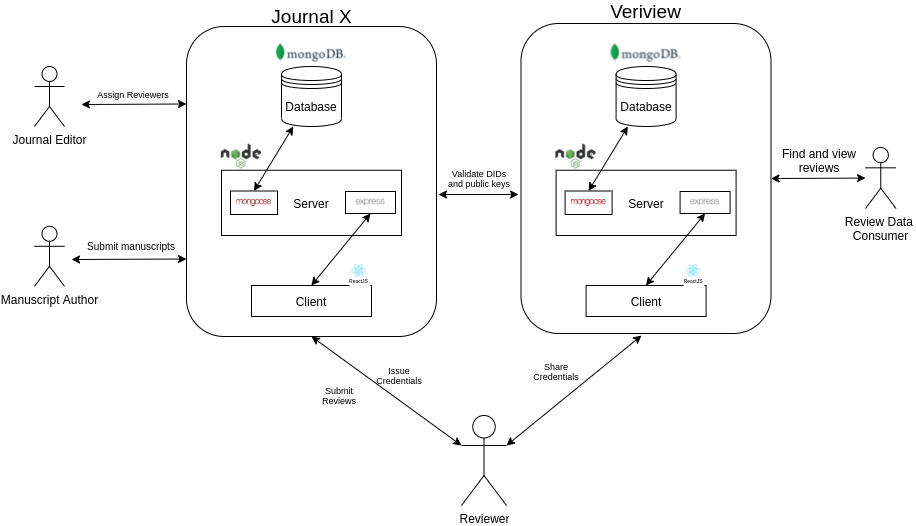
\includegraphics[width=0.8\textwidth]{figures/prototype.png}
  \caption{Overview of the architecture of the prototype} \label{fig:prototype}
\end{figure}

\subsection{Journal X}

Journal X is the simulated journal management system. Researchers can create an account an submit a manuscript to the journal. The prototype is deployed at \url{https://journalx.herokuapp.com}. The application is built on a \acrshort{MERN} stack. The MongoDB database stores the \lstinline{User} and login \lstinline{Token} data, in addition to the \lstinline{Manuscript}, \lstinline{Review}, and the \lstinline{ReviewTask} data. The \acrshort{CRUD} operations are done through the Mongoose driver that runs on the NodeJs Express server.

As the issuer identifier in the verifiable credentials, \acrshort{DID}s are used. The preferred \acrshort{DID} method is \lstinline{did:web} and the \acrshort{DID} of the implemented journal is \lstinline{did:web:journalx.herokuapp.com}. The document contains the public keys belonging to the journal that are used in credential verification. The \acrshort{DID} document is given in Listing \ref{lst:did-doc}.

\lstinputlisting[language=json, caption={Journal X \acrshort{DID} document},label={lst:did-doc}]{code/did-doc.json}

In Journal X, a researcher can view their manuscripts' statuses as in Figure  \ref{fig:submit-manuscript} and submit a manuscript that they want to be published in the form page upon clicking "Submit Manuscript". 

\begin{figure}[htpb]
  \centering
  
\includegraphics[width=0.8\textwidth]{figures/submitManuscript.png}
  \caption{View and Submit Manuscripts} \label{fig:submit-manuscript}
\end{figure}

Upon submission, a review process has been initiated for the manuscript. The editor can assign reviewers for the manuscript and change the publication status of the manuscript according to the reviews as in Figure \ref{fig:editor}. Users can see their assigned reviews (Figure \ref{fig:reviewer-screen}) and submit the review through the form page. The review includes an optional title, the content, an optional competing interest statement and a recommendation such as "Accept", "Minor Revision", "Major Revision" or "Reject". Finally they can see their submitted reviews as in Figure \ref{fig:view-review} and download the verifiable credential by clicking "Issue Credential".

\begin{figure}[htpb]
  \centering
  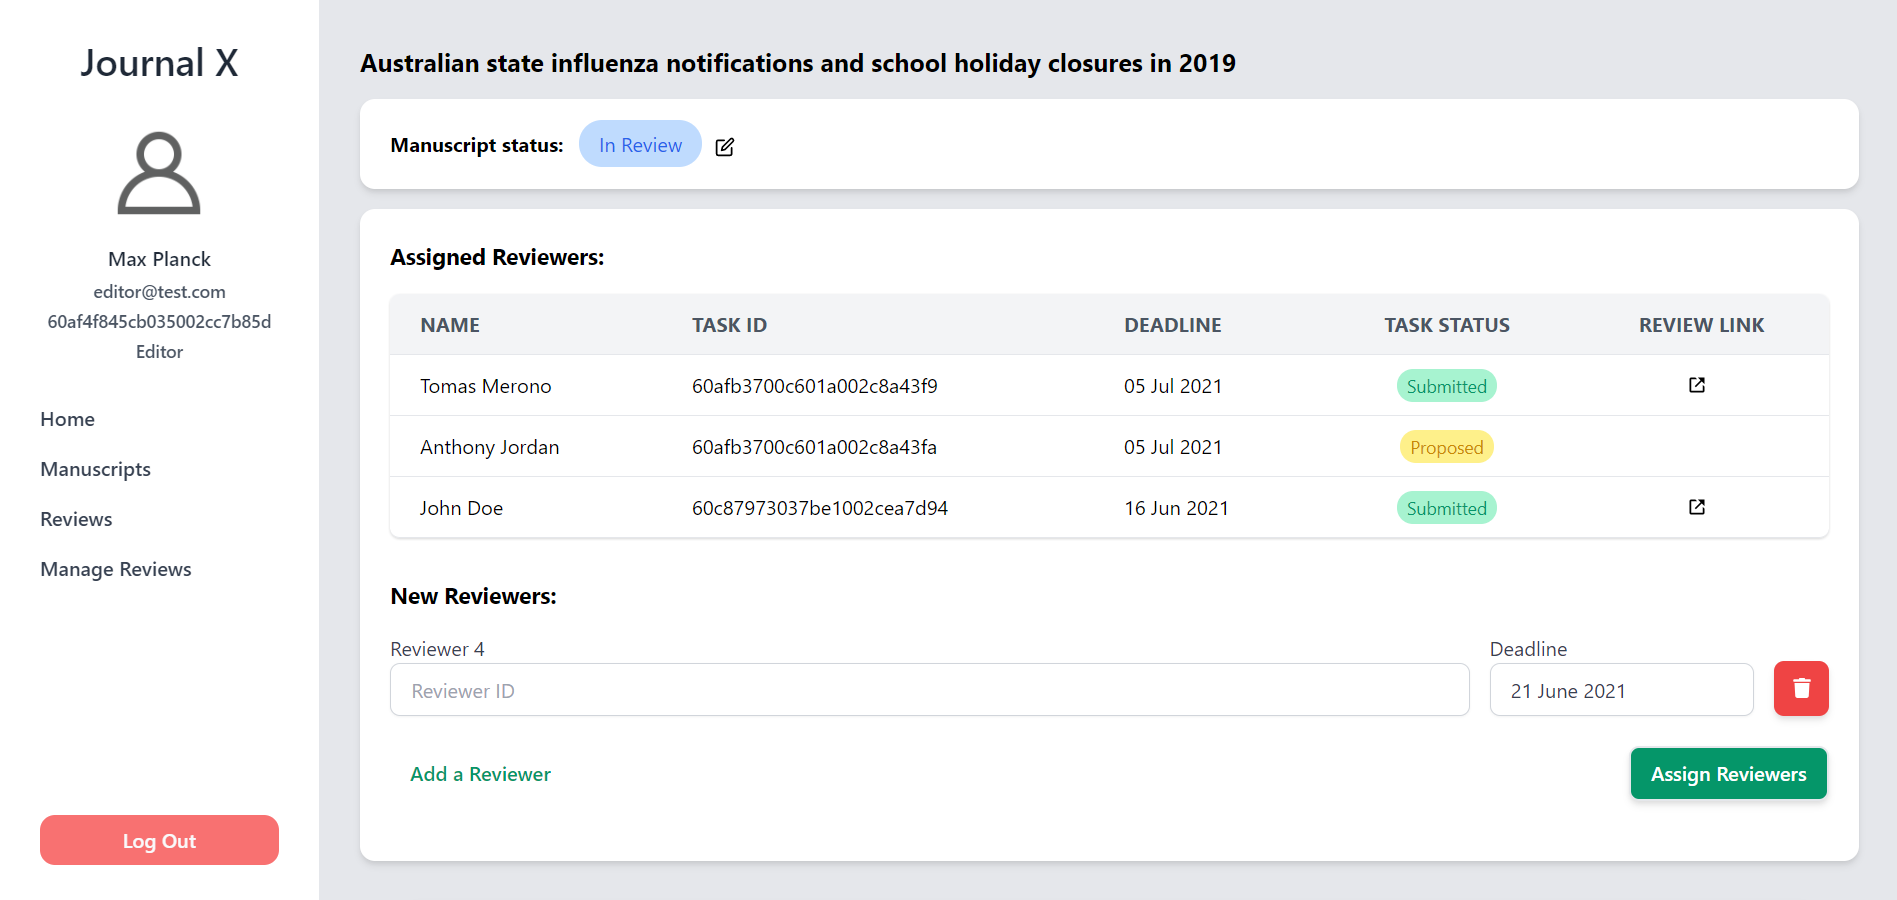
\includegraphics[width=0.8\textwidth]{figures/editor.png}
  \caption{Editor Manage Review Process Screen} \label{fig:editor}
\end{figure}

\begin{figure}[htpb]
  \centering
  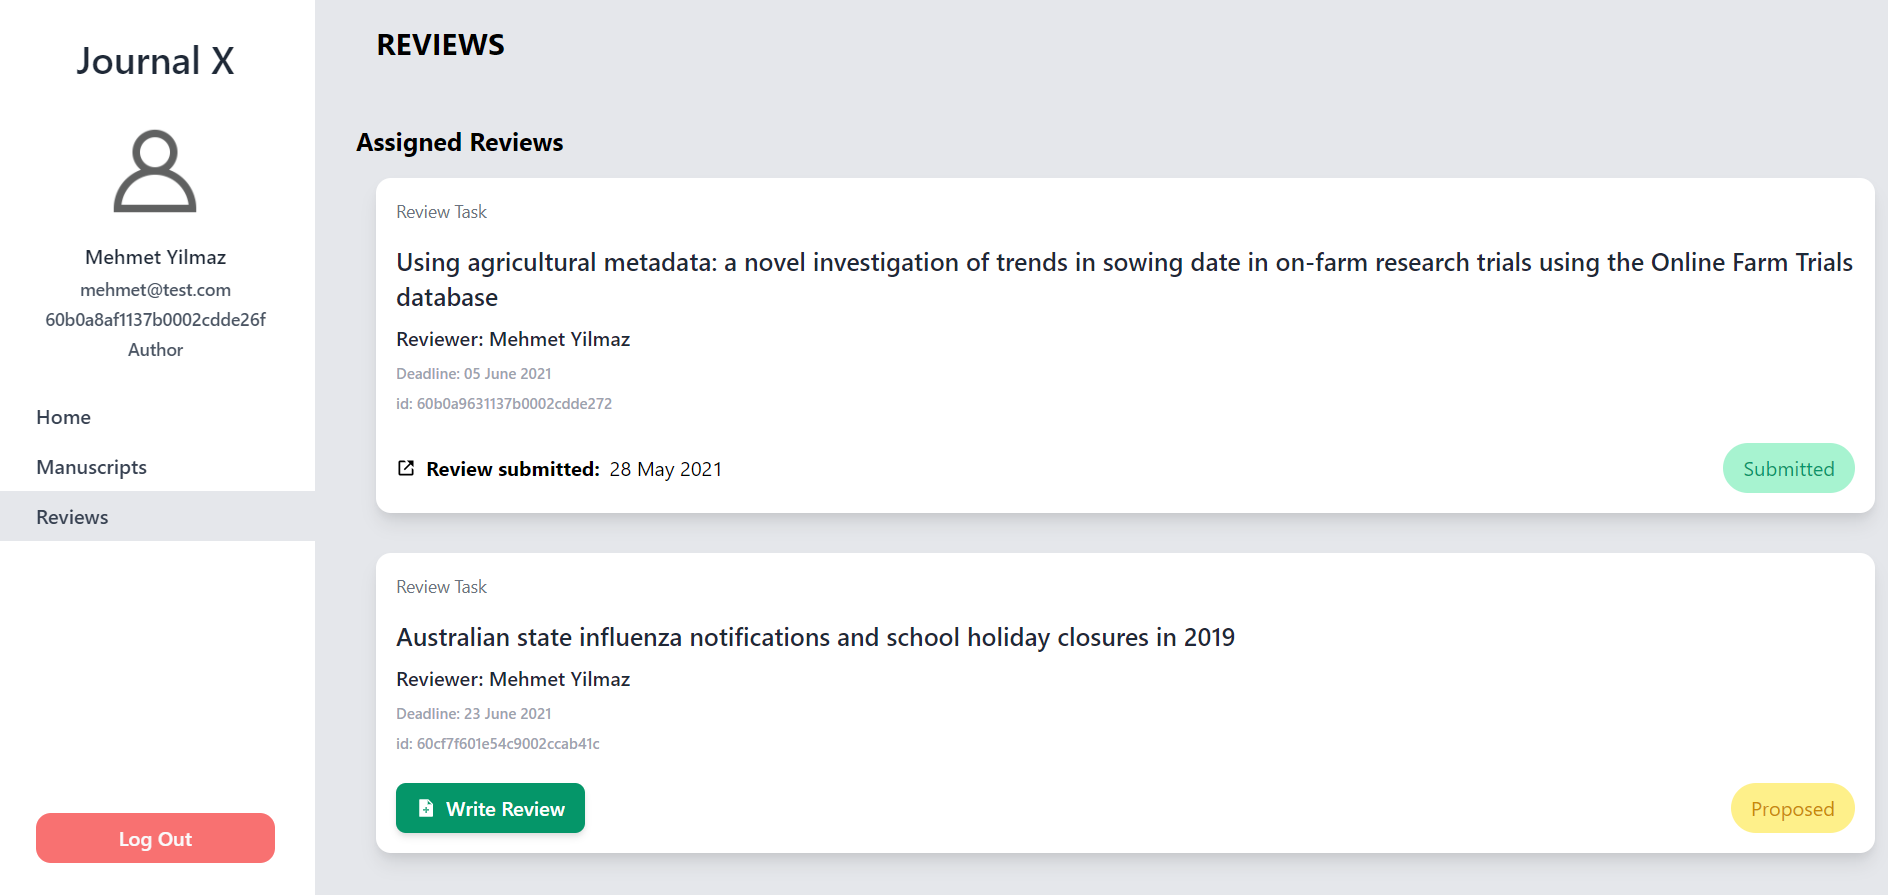
\includegraphics[width=0.8\textwidth]{figures/reviewerScreen.png}
  \caption{Reviewer dashboard} \label{fig:reviewer-screen}
\end{figure}

\begin{figure}[htpb]
  \centering
  
\includegraphics[width=0.8\textwidth]{figures/viewReview.png}
  \caption{View Review and Issue Verifiable Credential} \label{fig:view-review}
\end{figure}

When the credential is issued, it is downloaded to the reviewer's device as a file in \lstinline{.jsonld} format. Ideally these credentials are stored encrypted in a credential wallet or another dedicated application and only leave the application after deriving the credential. However, our prototype does not include a wallet since there are no existing ready to use wallet applications that support BBS+ signatures and credential derivation. Also, the credential exchange should be mediated by a secure protocol such as DIDComm\footnote{https://identity.foundation/didcomm-messaging/spec/}.  Instead, the users download their credentials plain text and use this file in the platforms. The secure connection is also out of scope of this work and only a HTTPS connection is established between the user and the platforms.

\subsection{Veriview}

Veriview is the conceived peer review showcasing platform of the prototype. Similar to Journal X, it is built on the \acrshort{MERN} stack. The working application is deployed at \url{https://veriview.herokuapp.com}. In addition to a journal account, the users need to create a Veriview account. Once they have an account, they can add the review credentials they obtained from journals to their Veriview profile. To add a peer review, the users are prompted to select the local credential file on their device. The input credential will be parsed and verified on the application. The verification at this stage is on the original credential, and the user will be able to derive a credential in the next steps. The application will first fetch the contexts (unless they are cached), and check the syntax of the document. Following, it will fetch the issuer document, which in our case is the Journal X's \acrshort{DID} document. Since it's a \lstinline{did:web} identifier, it will fetch the \acrshort{DID} document at \url{https://journalx.veriview.com/.well-known/did.json}. Next, the signature on the credential, which is under the attribute \lstinline{proof} will be validated against the public verification key of the \acrshort{DID} document. If all steps succeed, the document will be marked verified with a green check on top as in Figure \ref{fig:select-attributes}

\begin{figure}[htpb]
  \centering
  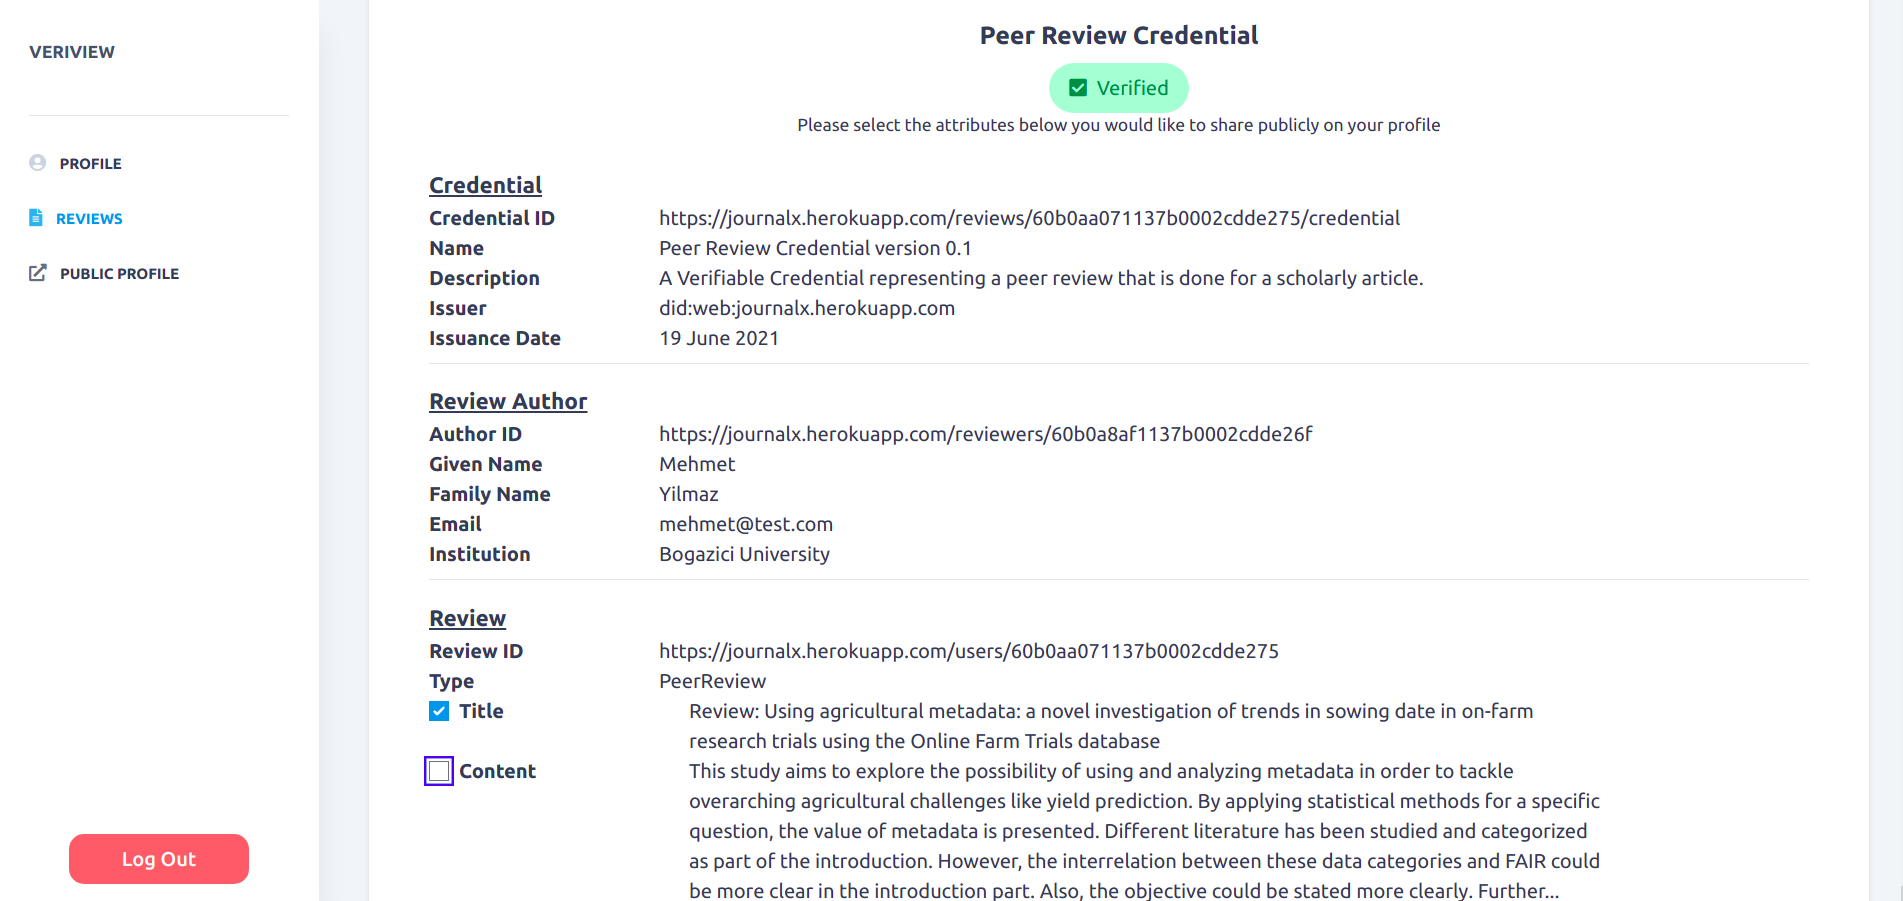
\includegraphics[width=0.8\textwidth]{figures/select-attributes.png}
  \caption{Adding the review credential to Veriview and selecting attributes} \label{fig:select-attributes}
\end{figure}

Here, the users can choose which attributes of a review they want to share publicly on their profile. For instance, typically a blinded review should not contain any information that would identify the review, meaning the review date, title, content, the manuscript title, and the manuscript abstract should be excluded. The interface does not allow users to exclude some fields such as the credential issuer, issuance date, review id, and review author information.

After selecting the attributes to be shared, a new credential will be derived from the original credential, which only contains the chosen attributes and a \lstinline{proof} attribute of type \lstinline{BbsBlsSignatureProof2020}. This proof is different than the signature of the original document, and is a zero-knowledge proof that the holder of this document knows a valid signature over the complete credential that is issued by the same issuer. The users can review the derived credential and add it to their profile by clicking "Submit". It is also possible to view the raw document in \acrshort{JSON-LD} format by clicking "Show Code", and download the derived credential (Figure \ref{fig:derived-credential}).

\begin{figure}[htpb]
  \centering
  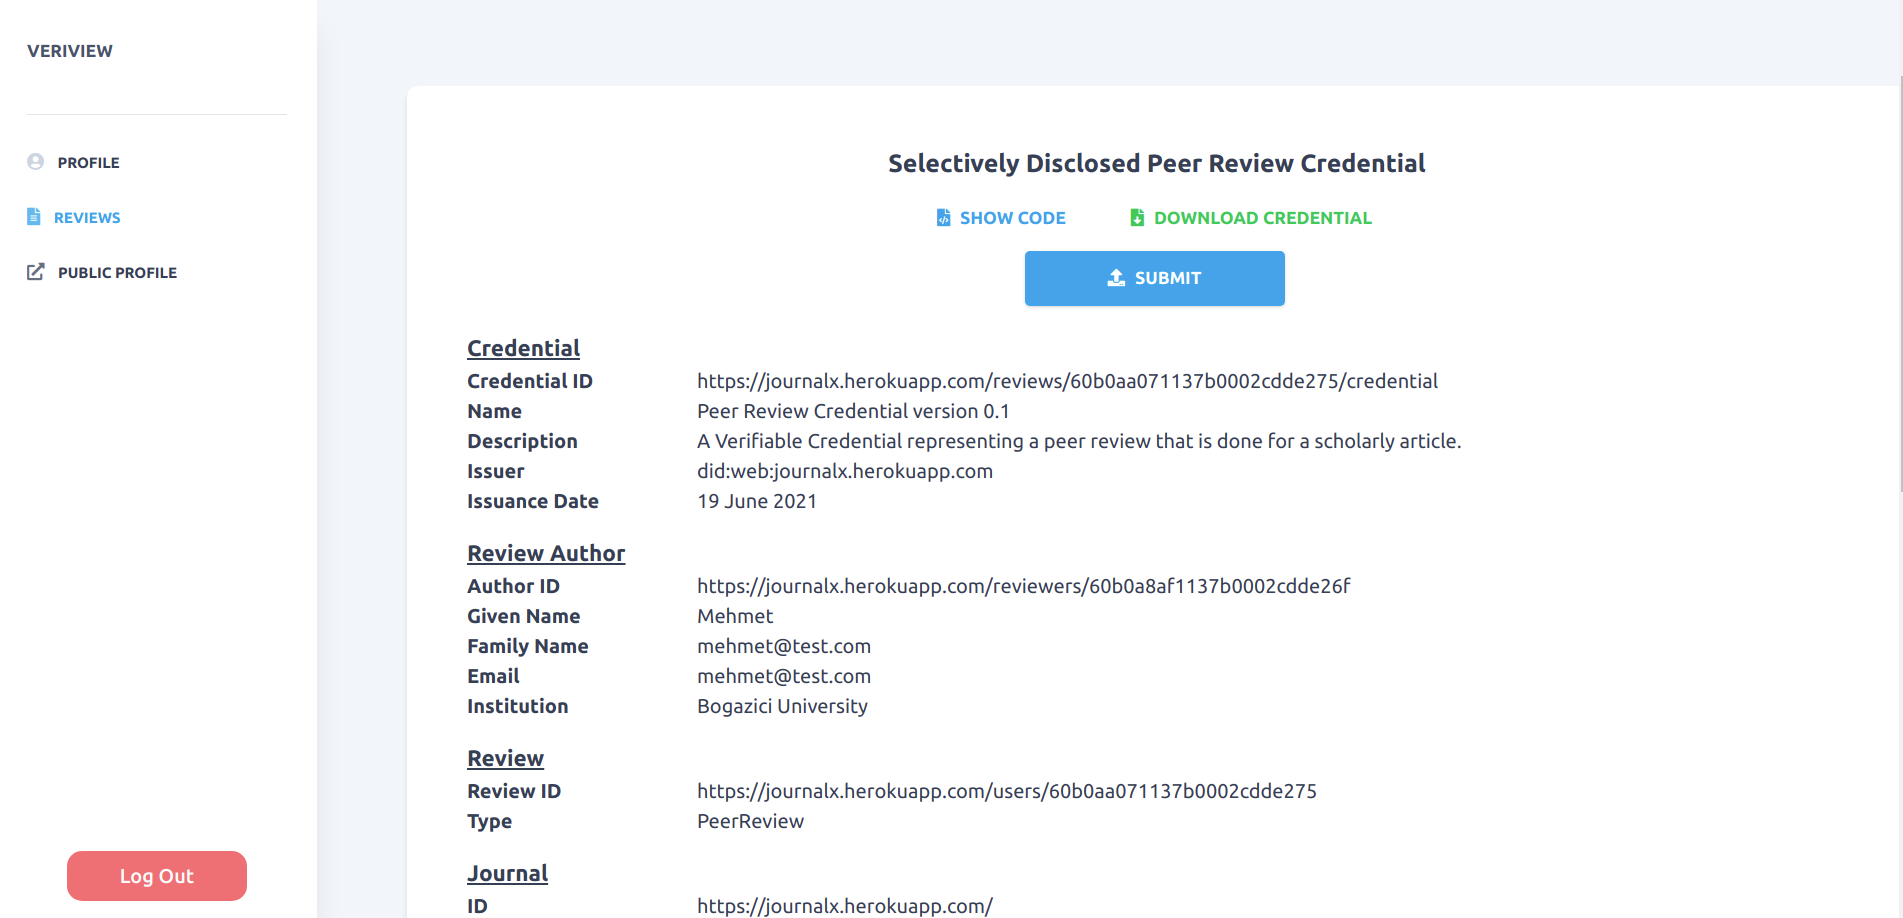
\includegraphics[width=0.8\textwidth]{figures/derived-credential.png}
  \caption{The selectively disclosed peer review credential} \label{fig:derived-credential}
\end{figure}

Finally users can view their profiles, and their profiles are publicly available at their unique \acrshort{URL}s. On this page the review consumers can view the review contributions of a researcher.

The prototype is not a complete implementation of the conceptual design and only serves the purpose of demonstrating the technical feasibility of the conceived system, in particular the \acrshort{VC} implementation of peer reviews including the issuance, verification of the credentials, and the selective disclosure with the zero-knowledge proofs. Table provides a comparison between the original design and the implemented prototype. 
% !TeX root = ../main.tex
% Add the above to each chapter to make compiling the PDF easier in some editors.

\chapter{Evaluation}\label{chapter:evaluation}

This section provides an evaluation of the designed artifact in two ways. In the previous section, seven requirements have been defined for the designed system. First, it will be discussed how the designed system fits in these requirements. Second, a qualitative evaluation of the system will be presented. For this part of the evaluation, one hour interviews with five different researchers with peer review experience were conducted. The \acrfull{TAM} is used as a framework to assess the system usage qualitatively. The responses by the interviewees are categorized under \acrshort{TAM} variables and interpreted to determine their intention to use of the system. According to the responses, a basic \acrlong{TAM} is proposed. Various insights gained during the interviews about the system and peer reviewing in general are also shared.

\section{Evaluation of Design Requirements}

Based on open science principles and the problems discussed, seven requirements were defined for the system:

\begin{itemize}
  \item RQ1: Verifiability 
  \item RQ2: Transparency 
  \item RQ3: Open Data 
  \item RQ4: Open Standards 
  \item RQ5: Direct Trust 
  \item RQ6: Selective Disclosure 
  \item RQ7: Compatibility 
\end{itemize}

\subsubsection{1. Verifiability}

Verifiability, in short, encompasses the ability to check if a peer review has really taken place and the presented information about the peer review is correct. The designed system is based on \acrlong{VC}, which makes use of the Linked-Data Proofs or \acrshort{JSON} Web Tokens that allows the verification of credentials using digital signatures. By resolving the \lstinline{issuer} (journal) identifier, their public keys can be retrieved and the credential can be verified. 

\subsubsection{2. Transparency}

The designed system improves upon the existing ones in numerous ways in terms of transparency. First of all, the verification of the peer reviews is transparent, that is anyone can take the existing data and verify that the peer review credential is actually issued by the given journal, and that it is authentic. Current showcasing platforms verify the reviews themselves and mark the reviews as verified without information on how this verification is done. Also, the Veriview platform can complete the verification steps and inform the users on its user interface that the review is verified. By open sourcing the code this process is also kept transparent.

\subsubsection{3. Open Data}

Even though the nature of blinded peer reviews prevents complete openness of the data, the system makes it possible to keep as much data of peer reviews as possible open without losing verifiability. Additionally, the data stored in Veriview is identical to what is publicly available. 

\subsubsection{4. Open Standards}

The system is based on open standards under development such as \acrlong{VC}, \acrlong{DID}, \acrshort{JSON-LD}. The platforms are open sourced and anyone can easily create a similar platform. This would avoid future vendor lock-in and further contributes the openness of the system.

\subsubsection{5. Direct Trust}

The peer review credentials are issued directly by journals and the verification is also done through journal keys. The showcasing system only serves as a platform to share and host the credentials, and requires minimal trust. 

\subsubsection{6. Selective Disclosure}

By using Linked-Data Proofs with BBS+ Signatures, it is possible to derive credentials with a subset of the attributes, and with a zero-knowledge proof that ensures the knowledge of the original credential and a valid signature. This enables review authors to only share the non-identifiable information of a review without losing verifiability.

\subsubsection{7. Compatibility}

The proposed system allows the extension of the proposed peer review vocabulary or the use of different vocabularies instead. This enables to accommodate the data model of the credentials to different peer review processes but also keeps the interoperability by having the vocabularies published. 

\section{Interviews}

For the qualitative evaluation of the work, 5 different researchers with peer review experience were interviewed: Interviewee 1, Kevin Wittek, Interviewee 3, Tiago Paixao, and Joao Oliviera. Interviewer 1 and Joao Oliviera were active Publons users and others have heard of it. The interviews took around 1 hour, were recorded and transcribed with the interviewees' consents. The interviews encompass first a general discussion around the interviewee's peer review experience and their perspectives, followed by an introduction to existing review showcasing platforms, in particular Publons, and their experience if they have any. Next, the conceptual design of the system is presented. The interviewees are then given a hands-on experience of the prototype and they are asked to complete the basic user flow of the application. Finally, their review of the system is solicited. 

The interviews were run as free dialogues and did not follow a strict structure besides the flow described above. However, the following or similar questions were asked to interviewees over the course of the interviews:

\begin{itemize}
    \item Could you please introduce yourself and detail your peer review experience?
    \item How would you describe the peer review culture in your field?
    \item What motivates you to do the peer review for a manuscript?
    \item Has there been a case where you presented your reviews in an academic resume, or that it would be beneficial if you could present it?
    \item Are you using review showcasing platforms? If yes, could you describe your experiences?
    \item What consequences may arise in the future that Publons is the only owner of the peer review data?
    \item Do you think the value added by Veriview exceeds the complexity it creates?
    \item What might be a reason to share or not to share your peer reviews on such a platform?
    \item Who might be interested in consuming the peer review data on Veriview?
\end{itemize}

A recurring theme across all interviewees was the lacking constructiveness and quality in some reviews and that some review authors don't seem to invest sufficient time to write reviews that will improve the manuscript. This seems to dishearten the researchers who try to write good reviews. Another discouraging experience mentioned by interviewees has been the cases where the interviewees see a paper they carefully reviewed with constructive feedback being published elsewhere without any of their input being taken into account. Nevertheless, all but one interviewees state reciprocity and a sense of duty as the main motivations to do peer reviews. The second common motivation stated has been the early access to research in their fields and having an idea what other researchers are working on. These are in line with the existing research and surveys \parencite{Publons.2018, Taylor&Francis.2015, Ware.2008, Squazzoni.2013}. 

Our interviewees all include their review or editorial work in their academic resumes, but usually this information is given a low priority without much detail and placed at the bottom of the resume. Because as Kevin Wittek stated: "there is not really a culture that the reviews become part of your CV or of your reputation". If this was the case, for instance reviewing in a high ranking journal would increase the reputation of scientists, then the reviewers would invest more resources to reviewing, he also explains. Tiago Paixao also affirms that these contributions are not deemed important. Interviewer 3 pointed out having this information on the resume demonstrates that you are connected with certain communities and having recently a best peer reviewer prize awarded, they became aware that it is nice to have this type of work published. Joao Oliviera brought the value of these records into question as it does not convey any information on the quality of the review and reminded that many reviewers don't really put much effort. Interviewee 1 mentioned that including this field shows that one engaged with the broader science, and it contributes to their periodical evaluations. But at the same time, institutions don't want researchers to spend much time doing peer review and their main focus is publications and grants a researcher has, and researchers' incentives are not aligned to do reviews but to publish papers and get grants, as Tiago Paixao mentioned. "The peer review is really, in objective terms, a waste of time. It's really an altruistic thing you do, I think", he said.

Even though most interviewees include peer reviews in their resume, some of them didn't think verification would be a necessity. "I'm sure people inflate their CV's" said Interviewee 1, "...but I don't think there's much incentive to lie with your peer reviews.". Interviewee 3 said they are not aware of anyone falsely claiming he/she reviewed for a journal, or if there's a motivation to do that. They also think Publons, despite being a trusted third-party, is not incentivized to publish inaccurate data as this is their core business and such an action would impair their reputation heavily. 

On the one hand, these statements show that researchers care for their peer review work and want to demonstrate their efforts but the larger scientific community doesn't seem to regard review service as a measure in practice. More visibility and availability of reviews would be a positive change for researchers in this sense. However, the perspectives on the unnecessariness of proofs, unimportance of reviews, and that no one would lie with their review work demonstrates the need for further validation of the significance of the problem.

When asked about Publons, our interviewees said they heard other people using it. The active users started using it after receiving an automatic invitation following a review they submitted, and they denote that they don't put much effort on their profiles, and actively add reviews. 

When questioning about the consequences of Publons being the only owner of the peer review data, we received contrasting answers. Our interviewees mostly expressed they didn't consider this before. 2 of the reviewers didn't see this as a problem, one even favored centralization that it brings more accountability and makes it easier to manage the data. Also, some interviewees don't consider that Publons has all the data but only the ones shared by the users, therefore that it does not strictly control the data and only collects a portion of it. However, concerns have been raised that if the platform becomes a de facto standard for review recognition, it could create a harder vendor lock-in, similar to what the scientific community experienced in the acqusition of Mendeley by Elsevier\footnote{https://www.mysciencework.com/omniscience/elsevier-takes-over-mendeley-and-you-what-do-you-think}. The fact that this data is controlled by a commercial entity is not necessarily bad, but something to be cautious of, especially that in the future this data can be monetized in various ways that won't be favored from an open science standpoint. We observe that for the interviewees with interest in open science practices and decentralization, this concern is expressly higher. Another decentralization aspect was brought up by Interviewee 3 that this may cause established reviewers to get more invitations and others less, and a more equal distribution of the review work is favored. Such inequalities are already apparent in peer review \parencite{Warne.2016, Publons.2018,Ware.2008, Hochberg.2009} and the use of this data for reviewer matching could exacerbate this. 

We also introduced our conceptual design to the interviewees and observed their understanding of the concept. A common confusion was around how the credentials are issued and how the verification works. However, without needing to explain the technical details, they were able to understand that the proof shows the authenticity and the integrity of the review, and that a credential with a subset of the attributes of the original credential can be created. All interviewees agree that the designed artifact as it is, is more complex than the existing platforms, but they could easily see that these complexities can be abstracted away from the user by a Researchgate plugin or similar (Interviewee 3) or automating the Veriview-journal interactions (Tiago Paixao). The Interviewee 1 and Joao Oliviera, both Publons users, emphasize the need of effortlessness on these steps. Since researchers, currently, don't put too much value on showing their reviews, these steps have to be as easy as possible. Kevin Wittek points out the typical learning curve in \acrshort{SSI} systems which includes making users aware that the credentials and keys are under their responsibility, and the cases of wallet loss and key management need to be considered. Even though in our system \acrshort{DID}s are not a requirement for authors, credential management can become a usability issue as stated. 

When asked who would become a review data consumer, journals and journal editors looking for reviewers were the common answers. Also, sometimes manuscript authors are asked to recommend reviewers and they can also benefit from the availability of this data, Kevin Wittek suggested. He also added researchers that need to regularly report their work can include their review efforts through systems like ours. Additionally, the Interviewee 3 stated such a platform can benefit researchers that would like to improve their writings and reviewing skills by providing access to good reviews. Institutions can also make use of this data to better asses the researchers and see their contributions to the larger community, Tiago Paixao suggested.

\section{Technology Acceptance Model}

The use of information technologies in workplaces and organizations has been increasing significantly, improving productivity across many aspects. Scientific publishing is no exception \parencite[132]{Ware.2015}. Understanding the adoption of new technologies, therefore, is a major research interest and an established field. The \acrlong{TAM} \parencite{Davis.1985, Davis.1989, Davis.1989b} became a widely used framework for explaining the user acceptance and its validity has been tested many times since over a quarter century \parencite{Marangunic.2015}. \acrshort{TAM} proposes the perceived usefulness and the perceived ease of use as the main determinants of the attitude toward using the technology which also influences the behavioral intention to use. \cite{Davis.1989b} also found out does not fully mediate perceived usefulness and the
perceived ease of use and it is removed from the model. The model is rather parsimonious in number of variables, and different extensions to the model have been proposed \parencite{Marangunic.2015}. 

\begin{figure}[htpb]
  \centering
  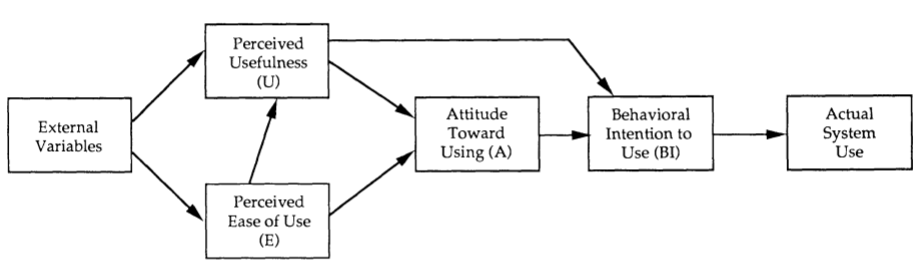
\includegraphics[width=0.8\textwidth]{figures/TAM.png}
  \caption{\acrlong{TAM} \parencite{Davis.1989b} } \label{fig:tam}
\end{figure}

Based on our findings from our interviews we discuss the variables that would influence the perceived usefulness and the perceived ease of use of our designed system by the users and propose a technology acceptance model. As users we consider only review authors but there are many potential types users such as journals, universities, research institutes etc. 

\subsection{External Variables}

\subsubsection{Significance of Reviews}

A common statement during the interviews was the insignificance of reviews in assessments, tenure, and overall researcher reputation. This was also apparent in how researchers include their review work in their resumes, by only sparing little space for this information. The disparity of this perception in the scientific community with the peer review's importance in scientific knowledge generation has been discussed in previous sections. The disparity has caught the attention of the community \parencite{Verissimo.2013, Tennant.2020} and the need for more recognition to peer review is being voiced. Researchers expect their institutions to require and recognize peer review contributions \parencite{Publons.2018} and state they would spend more time on reviews if it was recognized \parencite{Warne.2016}.

We define the variable broadly as significance of reviews, as this includes both the inherent value researchers give to reviews, the degree of recognition from institutions, and the attitude of the scientific community towards review work of a researcher. More significance of peer review works of a researcher would increase the need for such peer review showcasing and verification systems. We therefore propose that the significance of reviews will have a positive effect on the perceived usefulness of the technology. Interestingly, we argue, this is a chicken and egg problem, where the under-utilization of review recognition platforms are due to peer review's insignificance, and peer review's under-recognition is a result of unavailability of ways to demonstrate peer review work. Put other way, there exist the potential of a virtuous feedback loop: more visibility to peer review may foster peer review's significance and more significance of the process would create more demand to use showcasing platforms.

\subsubsection{Open Science Commitment}

Open Science Commitment can be defined as the degree of support of a researcher for open science practices. The designed artifact aims to remove trusted third parties from the review verification process and promote open data and transparency. This aspect is also the main differentiating property of the designed system from the existing ones. Taking this into account and based on our observations during the interviews, we propose that open science commitment of a researcher will have a positive impact on the perceived usefulness of the system. This factor would also influence the preference of a user between existing showcasing systems and our designed system. 

\subsubsection{Active Use Requirement}

The majority of the interviewees expressed the need for automation of the user actions on the platform. Researchers don't spend much time on their peer reviews once they write and submit it. As Interviewee 1 said, reviewers just do the review, send it, then move on to other tasks. They don't think about that review anymore. Joao Oliviera also highlighted the importance of effortless usage of the system, saying he also was invited to try an application similar to Reserachgate but did not continue using it as he didn't want to get into the trouble. Either the value added by the platform should be evident to put time on platform's tasks or it should be as effortless as possible. Google Scholar, since it is the primary online profile and shows a scientist's publications and citation metrics, is checked regularly by Interviewee 1 but they almost never spend time on their Publons profile. Based on these observations we propose that the active use requirement has a negative effect on the perceived ease of use. The most important component of this would be adding the reviews to the user profile. If this step could be automated, the perceived ease of use would highly increase.


\subsubsection{Institutional Demand}

warne: would spend more time on review if the institution recognizes

\subsubsection{Review Resume Eagerness}











% The Interviewee 1 and Joao Oliviera, both Publons users, emphasize the need of effortlessness on these steps. Since researchers, currently, don't put too much value on showing their reviews, these steps have to be as easy as possible. We can interpret this as the  
% !TeX root = ../main.tex
% Add the above to each chapter to make compiling the PDF easier in some editors.

\chapter{Discussion}\label{chapter:discussion}

Peer review is a controversial topic in science
many innovations fail
scientific publishing slow to change
too many stakeholders
This work 

First of all, our proposed system require journals to issue peer review credentials. This requirement is a major barrier for adoption as journals must be convinced of the value implementing such a would bring. Besides we assume a very simple peer review process. As discussed, the process varies a lot among journals. Even though the vocabularies are extensible, there need a degree of agreement to mutual vocabularies. Too much extensibility would break the interoperability in practice. 

Who maintains Veriview. What are the incentives? We say its open source and everyone can run veriview. What are the incentives to run in first place? If there are more than one showcasing platforms, then the data is scattered. 

Cold start problem. Bootstrap with existing peer reviews?

More validation of the practical relevance of review verification. and problem of publons. 

The system inherits the advantages of \acrshort{SSI} and \acrshort{VC} systems such as verifiability, selective disclosure... However, the problems of these systems are also inherited. Digital identity is a broader problem . Wallets.

We prefer not to use DLTs.

ok lets recognize reviews, but how? As joao underlines. Nevertheless, there's demand from community and as experiments like ours may reveal better ways
% !TeX root = ../main.tex
% Add the above to each chapter to make compiling the PDF easier in some editors.

\chapter{Conclusion}\label{chapter:conclusion}

In this work, we present a design science research on peer review recognition and deliver a system design as an artifact. Our work initially gives an overview of the peer review. We presented the problems discussed in the literature, and highlight the currently misaligned incentives to publish more and get cited more instead of doing peer reviews. Despite being considered highly important and essential in scientific knowledge generation, scientists are not incentivized to do peer reviews and there are concerns on the implications of this on the quality and the sustainability of the peer review. We further investigated the problem and described the lack of recognition for the peer review work of the researchers, and argued that this is partly caused by the nature of the practice of blinded reviewing, that requires identities to be hidden and reviews not to be published. We examined the existing platforms tackling this problem and identified current and future problems from an open science perspective. We observed that these platforms aggregate data by acting as trusted third-party peer review verifiers. From this specific problem we derived our research question:

\begin{center}
    \textit{How can closed peer reviews be verified without trusted third-parties?}
\end{center}

To answer this question we designed and developed a system using \acrlong{VC} and \acrfull{zk-proofs}. The designed system enables the verification of peer reviews through journals that issue peer review credentials. It also includes a review showcasing platform where reviewers can add these verifiable credentials without breaking the anonymity of the blinded reviews. We also implement a proof of concept prototype to show the technical feasibility of the conceptual design.

Our evaluation shows how we fulfil the self-imposed requirements but also demonstrates the need for further validation of our problem. 


% \appendix{}

% TODO: appendix chapter
% \chapter{General Addenda}

If there are several additions you want to add, but they do not fit into the thesis itself, they belong here.

\section{Detailed Addition}

Even sections are possible, but usually only used for several elements in, e.g.\ tables, images, etc.

\chapter{Figures}
\section{Example 1}
\cmark
\section{Example 2}
\xmark

\microtypesetup{protrusion=false}
\listoffigures{}
\listoftables{}
\microtypesetup{protrusion=true}
\printglossary[type=\acronymtype]
\printglossary
\printbibliography{}

\end{document}
